\chapter{Detector installation}
\label{ch:dp-installation}

\section{Introduction}
\label{ch:dp-install-intro}

This chapter covers the work and the infrastructure required to install the \dword{dune} \dword{dp} \dword{fd} module.
The infrastructure and the installation sequence have been defined assuming that the cryostat of the \dword{dpmod} is installed in an empty cavern.
This allows for more flexible installation of the needed infrastructure.
If the \dword{dpmod} is the third module installed, a different installation procedure and infrastructure should be defined.
This is out of the scope of this chapter.

A \dword{dune} \dword{fd} module has outer cryostat dimensions of $65.8 \times 18.9 \times 17.8$~m$^3$.
Every piece of the cryostats and the detectors must descend about 1500~m down the Ross shaft to the 4850-foot level of \dword{surf} and be transported to the detector cavern.
The installation of the detector is done in close collaboration with \dword{lbnf}, that is in charge of  excavating the caverns and providing the cryostats for all the \dword{dune} modules.

Inside the cryostat the \dword{dp} detector consists of:
\begin{itemize}
\item 80 $3 \times 3$~m$^2$ \dwords{crp} installed across the liquid/vapor argon interface.
\item  12 $12 \times 12$~m$^2$ \dword{fc} modules installed vertically along the walls.
\item  15 cathode modules  installed parallel to the \dwords{crp} and hanging from the bottom of the \dword{fc}.
\item  720 \dwords{pmt} installed on the cryostat floor under the cathode and a protection ground grid.
\item  A set of instruments to optimally operate the \dword{tpc} (purity monitors, temperature sensors, level meters, cryogenic cameras).
\end{itemize}

Compared to the \dword{spmod}, the installation of the \dword{dpmod} is significantly simpler inside the cryostat and it requires less complex infrastructure.
The sequence of installation is driven by the tests of the \dwords{crp}.
The work on the \dword{dpmod} can profit from all the infrastructure already in place for the installation on the \dword{spmod}, like the \dword{cuc}, the underground mechanical workshop, the storage facility, the logistic, and so on.

Some of the detector components arrive at \dword{surf} fully or mostly assembled, like the \dwords{crp}.
Others are mostly assembled underground, like the field cage modules.
The majority of the activities happen in a clean room, set up in front of the \dword{tco} entrance and inside the cryostat.
The clean room is equipped with four cold boxes where the \dwords{crp} go through the final cryogenic and HV tests.

After about twelve months of detector component installation, which follows twelve months of detector infrastructure installation, the cryostat is closed (with the last installation steps occurring in a confined space accessed through access ports on the roof). %, called man-holes).
Following leak checks, final electrical connection tests, the process of filling the cryostat with 17~kton of \dword{lar} begins.
The installation of \dword{dpmod} requires meticulous planning and execution of all the tasks by well trained teams of technicians, riggers, and detector specialists.

The high-level requirements for the \dword{dpmod} installation are summarized inTable~\ref{tab:specs:just:DP-INST}. 

% This file is generated, any edits may be lost.
\begin{footnotesize}
%\begin{longtable}{p{0.14\textwidth}p{0.13\textwidth}p{0.18\textwidth}p{0.22\textwidth}p{0.20\textwidth}}
\begin{longtable}{P{0.12\textwidth}P{0.18\textwidth}P{0.17\textwidth}P{0.25\textwidth}P{0.16\textwidth}}
\caption{Specifications for DP-INST \fixmehl{ref \texttt{tab:spec:DP-INST}}} \\
  \rowcolor{dunesky}
       Label & Description  & Specification \newline (Goal) & Rationale & Validation \\  \colhline

   
  \newtag{DP-INST-1}{ spec:handling-specs }  & Compliance with the material handling specification for all material transported underground  &  Fulfill material handling specification &  Being able to tranport undergound the equipment &  Material documentation and inspection \\ \colhline
     % 1
   
  \newtag{DP-INST-2}{ spec:material-buffer }  & Material buffer at the warehouse facility  &  >1 month &  Limit the impact of delivery delays on the installation schedule &  Regular report from the construction sites \\ \colhline
     % 2
   
  \newtag{DP-INST-3}{ spec:underground-storage }  & Material storage available underground  &  >4~\dshorts{crp} &  Limit the impact of rejected detector components on the installation schedule &  Dedicated space to store the detector component available undergorund in the vicinity of the clean room \\ \colhline
     % 3
   
  \newtag{DP-INST-4}{ spec:clean-room-specs }  & Cryostat and clean room environment  &  >ISO-8 &  Safe handling of the detector components and limit the radioactive background &  Regular air quality checks, constant air filtering, regular cleaning of the clean room and the cryostat, use of clean room equipment \\ \colhline
     % 4
   
  \newtag{DP-INST-5}{ spec:cold-box-cryo }  & Cold box cryogenics system  &  Independent operation of the four cold boxes &  Guarantee the needed flexibility in the tests &  Simultaneous operation of the cold boxes \\ \colhline
     % 5


\label{tab:specs:just:DP-INST}
\end{longtable}
\end{footnotesize}the table~\ref{tab:requirements}.


In all the planning and future work, the preeminent requirement in the installation process is safety.
The installation of the \dword{dp} module presents a multitude of hazards that includes manipulation of heavy loads, work in tight areas and confined spaces, and working at heights above the floor, use of chemicals (e.g., as cleaning agents), use of cryogens, tests involving \dword{hv}.

Mitigation of these hazards begins with the strong review efforts and definition of specific safety rules by \dword{esh} teams of \dword{sdsd} and \dword{surf}.
All installation team members, both on surface and underground, will undergo rigorous formal safety training.
Any team member can stop work at any time for safety purposes.
Further details of the overall \dword{dune} safety plan are provided in the Technical Coordination volume of \dword{tdr}.
In addition, each section of this chapter provides further details on the evolving safety plan for the \dword{dp} module installation.


The high level risks associated to the \dword{dpmod} installation are summarised in Table~\ref{tab:risks:DP-FD-INST}.


% risk table values for subsystem DP-FD-INST
\begin{footnotesize}
%\begin{longtable}{p{0.18\textwidth}p{0.20\textwidth}p{0.32\textwidth}p{0.02\textwidth}p{0.02\textwidth}p{0.02\textwidth}}
\begin{longtable}{P{0.18\textwidth}P{0.20\textwidth}P{0.32\textwidth}P{0.02\textwidth}P{0.02\textwidth}P{0.02\textwidth}} 
\caption[Risks for DP-FD-INST]{Risks for DP-FD-INST (P=probability, C=cost, S=schedule) More information at \dshort{riskprob}. \fixmehl{ref \texttt{tab:risks:DP-FD-INST}}} \\
\rowcolor{dunesky}
ID & Risk & Mitigation & P & C & S  \\  \colhline
RT-DPINST-01 & Personnel injury & Follow the safety rules in force. & L & L & H \\  \colhline
RT-DPINST-02 & Cryostat damage during installation & Use temporary protection for the corrugated membrane. & L & L & M \\  \colhline
RT-DPINST-03 & Detector components damage during transport/installation & Handling should be done by trained people, following the handling instructions provided by the consortia and in presence of a technical expert. & L & M & M \\  \colhline
RT-DPINST-04 & Detector components failure during test & Only trained people should test equipments. Spare components must be available at the warehouse facility. & L & L & M \\  \colhline
RT-DPINST-05 & Components interferences & 3D model, survey at the construction sites, and full scale assembly tests. & M & L & L \\  \colhline
RT-DPINST-06 & Shipping delays/missing parts & Buffer material and detector components at the warehouse facility and use inventory tools to follow the fundamental items. & L & L & L \\  \colhline
RT-DPINST-07 & Lack of specialised/trained manpower & Hire and train personnel. Plan with all the underground stakeholders enough in advance the required personnel. & L & L & L \\  \colhline

\label{tab:risks:DP-FD-INST}
\end{longtable}
\end{footnotesize}



Access to the underground installation area for \dword{lbnf}, \dword{dune}, and \dword{jpo} personnel, as well as for \dword{lbnf} and \dword{dune} materials and equipment, will be provided by a single shaft, the mile-deep Ross Shaft.
Coordinating transport and ensuring on-time delivery of all items are therefore among the more challenging aspects of the \dword{lbnf} and \dword{dune} endeavor.
The \dword{jpo} will establish a logistics organization for \dword{lbnf} and \dword{dune}, operated under the \dword{sdsd}, to verify deliveries to the point of receipt in South Dakota and coordinate transport of materials from there to the Ross Headframe.

Due to the cost of the \dword{cf} contracts and the risk of increased construction costs due to delays in delivery of materials, the shaft scheduling must be tightly controlled by \dword{lbnf}-\dword{cf} during construction.
The shaft is outfitted with a hoist that controls the cage and the skips.
The cage is used to transport people, equipment and materials, and the skips are used to bring up muck and transport over-sized equipment and materials.
The \dword{lbnf}-\dword{cf} \dword{cmgc} will coordinate overall usage of the Ross Shaft during this period.
To facilitate the flow of materials and equipment not related to \dword{cf} through the Ross Headframe, the \dword{jpo} will lease a warehouse facility within a maximum one-day roundtrip from \dword{surf} by truck.
It is expected that the lease of this facility, referred to as the \dword{sdwf}, will include warehouse space, personnel, and \dword{wms} to inventory all incoming materials and equipment.
The location and the premisses  of the facility have not yet been identified.
Most detector and materials and equipment will be shipped to the \dword{sdwf}.
\dword{cf} material and cryogenics equipment are exceptions and will ship directly to \dword{surf}.

The \dword{sdsd} logistics organization will receive and inventory all goods shipped to the \dword{sdwf}, coordinate with the \dword{cmgc} and transport the material to the Ross Headframe in a just-in-time manner, and transport it underground and into the cavern.
The \dword{sdsd} logistics team oversees transportation of the cryostat (steel, foam, and membrane), the cryogenics system, the detector, and all related infrastructure not provided by the \dword{cf}.
\dword{lbnf} specifically oversees the cryostat and cryogenics system, which are discussed in detail in the \dword{lbnf} \dword{tdr}.
The space in the \dword{sdwf} must be shared between the detector components for the \dword{dpmod} and the \dword{lbnf} material to construct the next cryostat.

The \dword{surf} Facility Access Specification~\cite{bib:docdb328} defines the limitations on dimensions and weights for all materials to be transported underground, the most stringent of which are set by the Ross Shaft and Cage.
It is possible to bring material down the shaft underneath the cage or in the skip compartment as a slung load, but this is a much slower process and requires careful planning and review of detailed procedures for each trip.
In some cases this is the only possibility.
Most material will be brought underground inside the cage.
Figure~\ref{fig:shaft-cage} illustrates the new Ross Cage and summarizes its main dimensions.
\begin{dunefigure}[Ross Shaft cage]{fig:shaft-cage}
{Preliminary model of the new Ross Shaft cage.}
\includegraphics[width=1.\textwidth]{shaft-cage.png}
\end{dunefigure}

The roundtrip travel time for the Ross cage is 17 minutes, dominated by loading and unloading time (the actual travel time is 3.6 minutes each way).
Slung loads will require more than an hour round trip.
The Ross Headframe has no loading dock so careful planning of material loading and unloading of shipments is required.
All materials must arrive on a flatbed or curtain-sided chassis, and a
forklift will be available for unloading.
All deliveries, either from the \dword{sdwf} or direct to the Ross Headframe, require (1) coordination with the \dword{sdsd} logistics organization, and (2) minimum two weeks prior notice, per an advance delivery plan.
Logistics will provide a shipping manual to \dword{dune} institutions that will specify guidelines on required shipping data and cargo consignment such that the logistics organization can monitor shipping progress and no delays occur due to incomplete or missing documentation.
To prevent delays due to missing deliveries a minimum one month buffer of materials from detector components is foreseen.
This buffer will allow advance planning for the underground work, with confidence that all materials will be available as needed.
Sufficient space must be made available at the \dword{sdwf} and in the underground area to house this material.
To determine the storage space requirements and how much hoist time must be dedicated a detailed inventory of all detector equipment and infrastructure is needed.
The \dword{sdwf} staff in some occasion may de-consolidate or consolidate arriving cargo into appropriately sized boxes and crates, as needed, for delivery to \dword{surf}, to make the most efficient use of available trucks and the Ross Shaft.

The \dword{uit} supports the consortia installation effort and coordinates all the \dword{dune} underground work.
Each consortium is at all times responsible for the detector components and equipment that they provide to \dword{dune}.
The \dword{uit} supports the consortium installation work by providing the needed expertise to operate all cranes, platforms, hoists, and other specialized rigging equipment needed to move consortia equipment.
Special lifting devices are expected to be needed to install \dwords{crp}, \dword{hv} system \dword{fc} and cathode, and electronics.
Special devices may need to go through approval procedures and tests prior their use (tests that should be done on surface in the \dword{sdwf}).
The \dword{uit} leader is the responsible for supervising the \dword{uit} members, but the ultimate responsibility for all detector components will remain within the consortia even while the underground team is rigging or transporting these components.
This will be critical in case parts are damaged during transport or installation, as the consortia need to judge the necessary actions.
For this reason, a consortium representative or point of contact must be present when any work is performed on their equipment.
The consortium is also responsible for certifying that each installation step is properly performed.
The \dword{uit} is responsible for planning the work underground and communicating this plan to the consortia.
The consortia are responsible for planning the individual installation steps for their equipment and communicating this to the \dword{uit}.
This includes the reviewed and approved Consortium Installation Plan and all of the approved detailed Installation Procedures.



The installation requires meticulous planning and execution of thousands of tasks by well trained
 teams of technicians, riggers, and detector specialists. High-level requirements for these tasks are spelled out in %%%%%

%\cleardoublepage

\section{Detector infrastructure}
\label{ch:dp-tc-infrastructure}

The detector infrastructure for the \dword{dpmod} comprises the equipment used by several groups and consortia to install and operate the detector.
It includes the electronics racks on top of the mezzanine on the cryostat roof and the related networking, electrical and cooling power, cable trays, cryostat penetrations and flanges, detector ground isolation transformers, and monitors.
Inside the cryostat, the detector infrastructure includes the gas and liquid argon distribution manifolds, the cryostat false floor to protect the corrugated membrane and allow safe circulation of material and people inside the cryostat, movable scaffold and man lifts for activities at height, and the ventilation and air circulation and filtration.
A cleanroom equipped with  \coldbox{}es for the functional tests of the \dwords{crp} is also present in front of the \dword{tco}.
This cleanroom and the cryostat itself are the places where some detector components are manipulated and assembled before installation.

\subsection{Cryostat Roof}
The roof of the \dword{dpmod} cryostat is going to be very dense with equipment, more so than the \dword{spmod}.
Ideally all the roof surface that is not equipped with feedthroughs and racks should be walkable.
For this reason, at the same height of the cryostat I-beams, a floor capable of standing at least 250~kg/m$^2$ is installed.
The floor is not meant to move heavy material around the roof.
The material of the floor must comply with the safety rules in force.
Plywood painted with flame retardant agents may be a cost-effective and adequate option; that must be confirmed with \dword{esh}.
No pipes, tubing, or cable trays along the length or the width of the cryostat should be installed above the false floor, in order to minimize the risk of accidents to personel and material due to tripping.
The floor must segmented in sections that are easily opened by one person to allow easily access to the equipment underneath.
The most convenient passage to cross the entire length of the cryostat will be under the detector rack mezzanine.
Lighting under the cryogenics and the detector mezzanines will be available.
During cryostat construction, welding of the pipes and flanges, and installation of the cable trays, the false floor must be installed only in the zones dedicated to the passage, considering that the co-activity during these periods is expected to be high and each worker should have enough space to safely work and move.

A drawing of the full cryostat roof with its penetrations is shown in Figure~\ref{fig:DP-roof-penetration}.
A zoom of the same image of a corner on the opposite side of the \dword{tco} is shown in Figure~\ref{fig:DP-roof-penetration-zoom}.
The same figure shows also the \threed model of the roof with equipment on the \dword{crp} support and \dword{sgft} penetrations.
This image highlights the high density of the equipment on the \dword{dpmod} roof, even more important considering that each of these flanges will be reached by several cables.

\begin{dunefigure}[Drawing of \dshort{dpmod} roof]{fig:DP-roof-penetration}
{Drawing of the cryostat roof with its penetrations.}
\includegraphics[width=0.9\textwidth]{DP-roof-penetration.png}
\end{dunefigure}

\begin{dunefigure}[Zoom of the \dshort{dpmod} roof]{fig:DP-roof-penetration-zoom}
{Zoom of the \dword{dpmod} roof drawing (left) and 3D model of the same portion of the roof with the \dword{sgft} and \dword{crp} suspension chimneys instrumented.}
\includegraphics[width=0.45\textwidth]{DP-roof-penetration-zoom.png}
\includegraphics[width=0.45\textwidth]{DP-roof-penetration-3D.png}
\end{dunefigure}

The role of the roof penetrations is to connect the ultra-pure argon volume to the atmosphere through the roof insulation, while minimizing the heat input.
All the penetrations are on the roof of the cryostat except the ones for the liquid argon re-circulation that are at the bottom of the \dword{tco} wall.
The sketch of a typical roof penetration cross-section is shown in Figure~\ref{fig:penetration-cross-section-sketch}.
\begin{dunefigure}[Sketch of a typical roof penetration]{fig:penetration-cross-section-sketch}
{Sketch of a typical roof penetration.}
\includegraphics[width=0.9\textwidth]{penetration-cross-section-sketch.png}
\end{dunefigure}
The thermal insulation is installed around a vertical stainless steel pipe that is mechanically connected to the walls of the warm structure.
The corrugated membrane is welded vacuum tight to the pipes.
The excess pipe inside the cryostat volume may be used to weld a mechanical support, for instance to attach cable trays.

On the atmospheric side a \dword{uhv} CF flange is welded vacuum tight to the pipe.
Except for the four access ports, all the flanges on the chimneys follow the \dword{uhv} CF flange standard ISO 3669:2017.
The leak rate of this widespread standard vacuum connections is lower than $10^{-9}$~mbar$\times$L/s.
The feedthroughs and the mating flanges are expected to be compatible with this level of leaks.
All the penetrations, the flanges, and the feedthroughs will be leak tested in situ after the final installation with helium sniffing techniques sensitive to local leaks of $10^{-6}$~mbar$\times$L/s.
More sensitive techniques (like vacuum bags) may be applied to selected feedthroughs and penetrations if required.

The welded flanges on the roof may need to be supported in case they must sustain significant load, as for example in the case of the penetrations for the \dword{crp} and field cage supports.
These flanges carry out the role of interface between the cryostat and the feedthroughs.
The scope of the detector infrastructure ends at the flange.
Copper gaskets, bolts, and nuts are in the scope of the mating flange or feedthrough.
The holes for the bolts on the cryostat flanges are not threaded.
Special nuts may be needed if the support/reinforcement structure underneath the flange makes the tightening of the bolts too difficult.

In order to allow an effective air purge, each penetration will be outfitted with an exhaust. Each penetration is therefore equipped with 12~mm outer diameter pipes welded on the tube penetration.
This pipe is then connected to the main purge manifold by means of stainless steel flexible tubes.
The exhaust should be positioned high enough in order to minimize air pockets.
If the feedthrough extends significantly in the vertical direction form the roof flange, it is preferred that the exhaust is placed on the feedthrough flange itself.
The connection to the manifold is done in the same way with flexible tubing, while the exhaust welded on the penetration tube is vacuum sealed with the proper tube plug.

During the cryostat purging, the gas from the roof penetrations is exhausted through the dedicated pipes provided by the cryogenics system.
It is sampled with oxygen, nitrogen, and moisture analysers in order to define the argon gas purity.
This measurement determines the \cooldown and  filling process starts.
During operation, instead, the majority of the argon from the roof penetration is purified and re-condensed.
A fraction of it is analysed in order to study the internal sources of pollution (for instance cables) and to reveal the appearance of leaks.

On/off valves pneumatically controlled by the cryogenics control system are installed between the exhaust manifold and the penetrations.
A single valve may collect the flow from multiple neighboring penetrations.
The number of valves and the pattern of interconnections will be defined later also taking into account budget constraints.
The role of these valves is twofold: (1) They are used to isolate the gas flow from few selected penetration in order to study the location of the internal pollution sources. (2) They are used during the leak tests of the feedthroughs to feed helium gas in the chosen penetrations.

There are several kinds of penetrations that serves different needs.
Table~\ref{tab:penetrations} summarizes all of them.
\begin{dunetable}[Types of penetrations through the roof]
{cccccc}
{tab:penetrations}
{Types of penetrations through the roof.}
Type & Number & CF & Pipe ID (mm) & Ext. Sup. & Int. Sup.\\
\toprowrule \dword{crp} sup. & 240 & CF100 & 100 & yes & no\\
\colhline Field cage sup. & 24 & CF150 & 150 & yes & no\\
\colhline \dword{crp} inst. & 42 & CF250 & 250 & no & yes\\
\colhline Tank inst. & 20 & CF250 & 250 & no & yes\\
\colhline \dword{sgft} & 240 & CF275 & 267 & yes & no\\
\colhline VHV & 1 & CF250 & 250 & no & yes\\
\colhline Manhole & 4 & custom & 700 & no & no\\
\colhline Cryo & 39 & various & various & various & various\\
\end{dunetable}
\begin{comment}
\begin{dunetable}[Types of penetrations through the roof]
{ccccccc}
{tab:penetrations}
{Types of penetrations through the roof.}
Type & Number & CF & Pipe OD (mm) & Pipe ID (mm) & Ext. Sup. & Int. Sup.\\
\toprowrule \dword{crp} sup. & 240 & CF100 & 104 & 100 & yes & no\\
\colhline Field cage sup. & 24 & CF150 & 154 & 150 & yes & no\\
\colhline \dword{crp} inst. & 42 & CF250 & 254 & 250 & no & yes\\
\colhline Tank inst. & 20 & CF250 & 254 & 250 & no & yes\\
\colhline \dword{sgft} & 240 & CF275 & 273.2 & 267 & yes & no\\
\colhline VHV & 1 & CF250 & 254 & 250 & no & yes\\
\colhline Manhole & 4 & custom & 706 & 700 & no & no\\
\colhline Cryo & 39 & several & several & several & several & several\\
\end{dunetable}
\end{comment}
Interface documents stating the requirements and the constraints on the internal diameter of the penetration tube, on its linearity and verticality, and on the horizontality and orientation of the welded flanges will be agreed with the \dword{dune} consortia and the cryogenics.
The experience gained with \dword{pddp} showed that the most critical penetrations in this respect are the ones of the \dword{sgft}.
For this reasons, the internal dimension of the \dword{sgft} penetration pipes was increased to 267~mm.
The pipes of the penetration for the \dword{crp} suspensions are also increase to 100~mm internal diameter.

Table~\ref{tab:load-penetration} summarizes the penetration flanges subjected to significant mechanical loads for different conditions.
These require external supports.
\begin{dunetable}[Load for mechanical support penetrations]
{cccc}
{tab:load-penetration}
{Load for mechanical support penetrations.}
Type & Number & Empty (kg) & Full (kg) \\
\toprowrule \dword{crp} sup. & 240 & 150 & 150\\
\colhline Field cage sup. & 24 & 1100 & 700 \\
\colhline \dword{sgft} & 240 & 120 & 120 \\
\end{dunetable}

The support system for the \dwords{crp} is described in the \dword{crp} chapter of this \dwords{tdr}.
Each \dword{crp} is suspended at three points connected to the external \dword{crp} supports through the chimneys.
During \dword{crp} installation this system allows attachment of the \dwords{crp} at the level of the cryostat internal floor followed by lifting them up to their final position.
In this condition, the system allows manual horizontal adjustment of $\pm 26$~mm and electrically controlled vertical adjustment of $\pm 40$~mm.
The vertical movement is used to adjust the horizontality of the height of the \dwords{crp} with respect to the \dword{lar} level.
The horizontal movement allows minimization of the uninstrumented surface arising from the thermal shrinkage of the \dwords{crp}.
The cryostat structural I-beams are spaced every 1.6~m, while the \dword{crp} size is $3\times3$~m$^2$.
In order to avoid interference between the I-beams and the \dword{crp} support system, the position hanging points is not always the same for all the \dwords{crp}.
There are two different triangular patterns and the \dword{crp} structure copes with boths.
The \dword{crp} will have different hancoring points to meet the different positions of the penetrations.

The heaviest load that this system must withstand is during the lifting of the \dwords{crp} and the opening of the protection box.
The estimated load for each penetration in this condition is 240~kg.
Square steel tubes solidly welded to the cryostat main I-beams will support the weight.
Analogous reinforcement are expected for the field cage support penetrations.
These reinforcement are installed at the same time when the flanges will be welded on the penetration pipes.
The detailed design of these elements is not defined yet.
The equivalent implementation of the supports in \dword{pddp} is shown in Figure~\ref{fig:mechanical-supports}.
\begin{dunefigure}[Mechanical support of the \dshort{crp} and \dshort{fc} support penetrations in \dshort{pddp}]{fig:mechanical-supports}
{Photos of the mechanical support of the \dword{crp} (left) and field cage (right) support penetrations implemented in \dword{pddp}.}
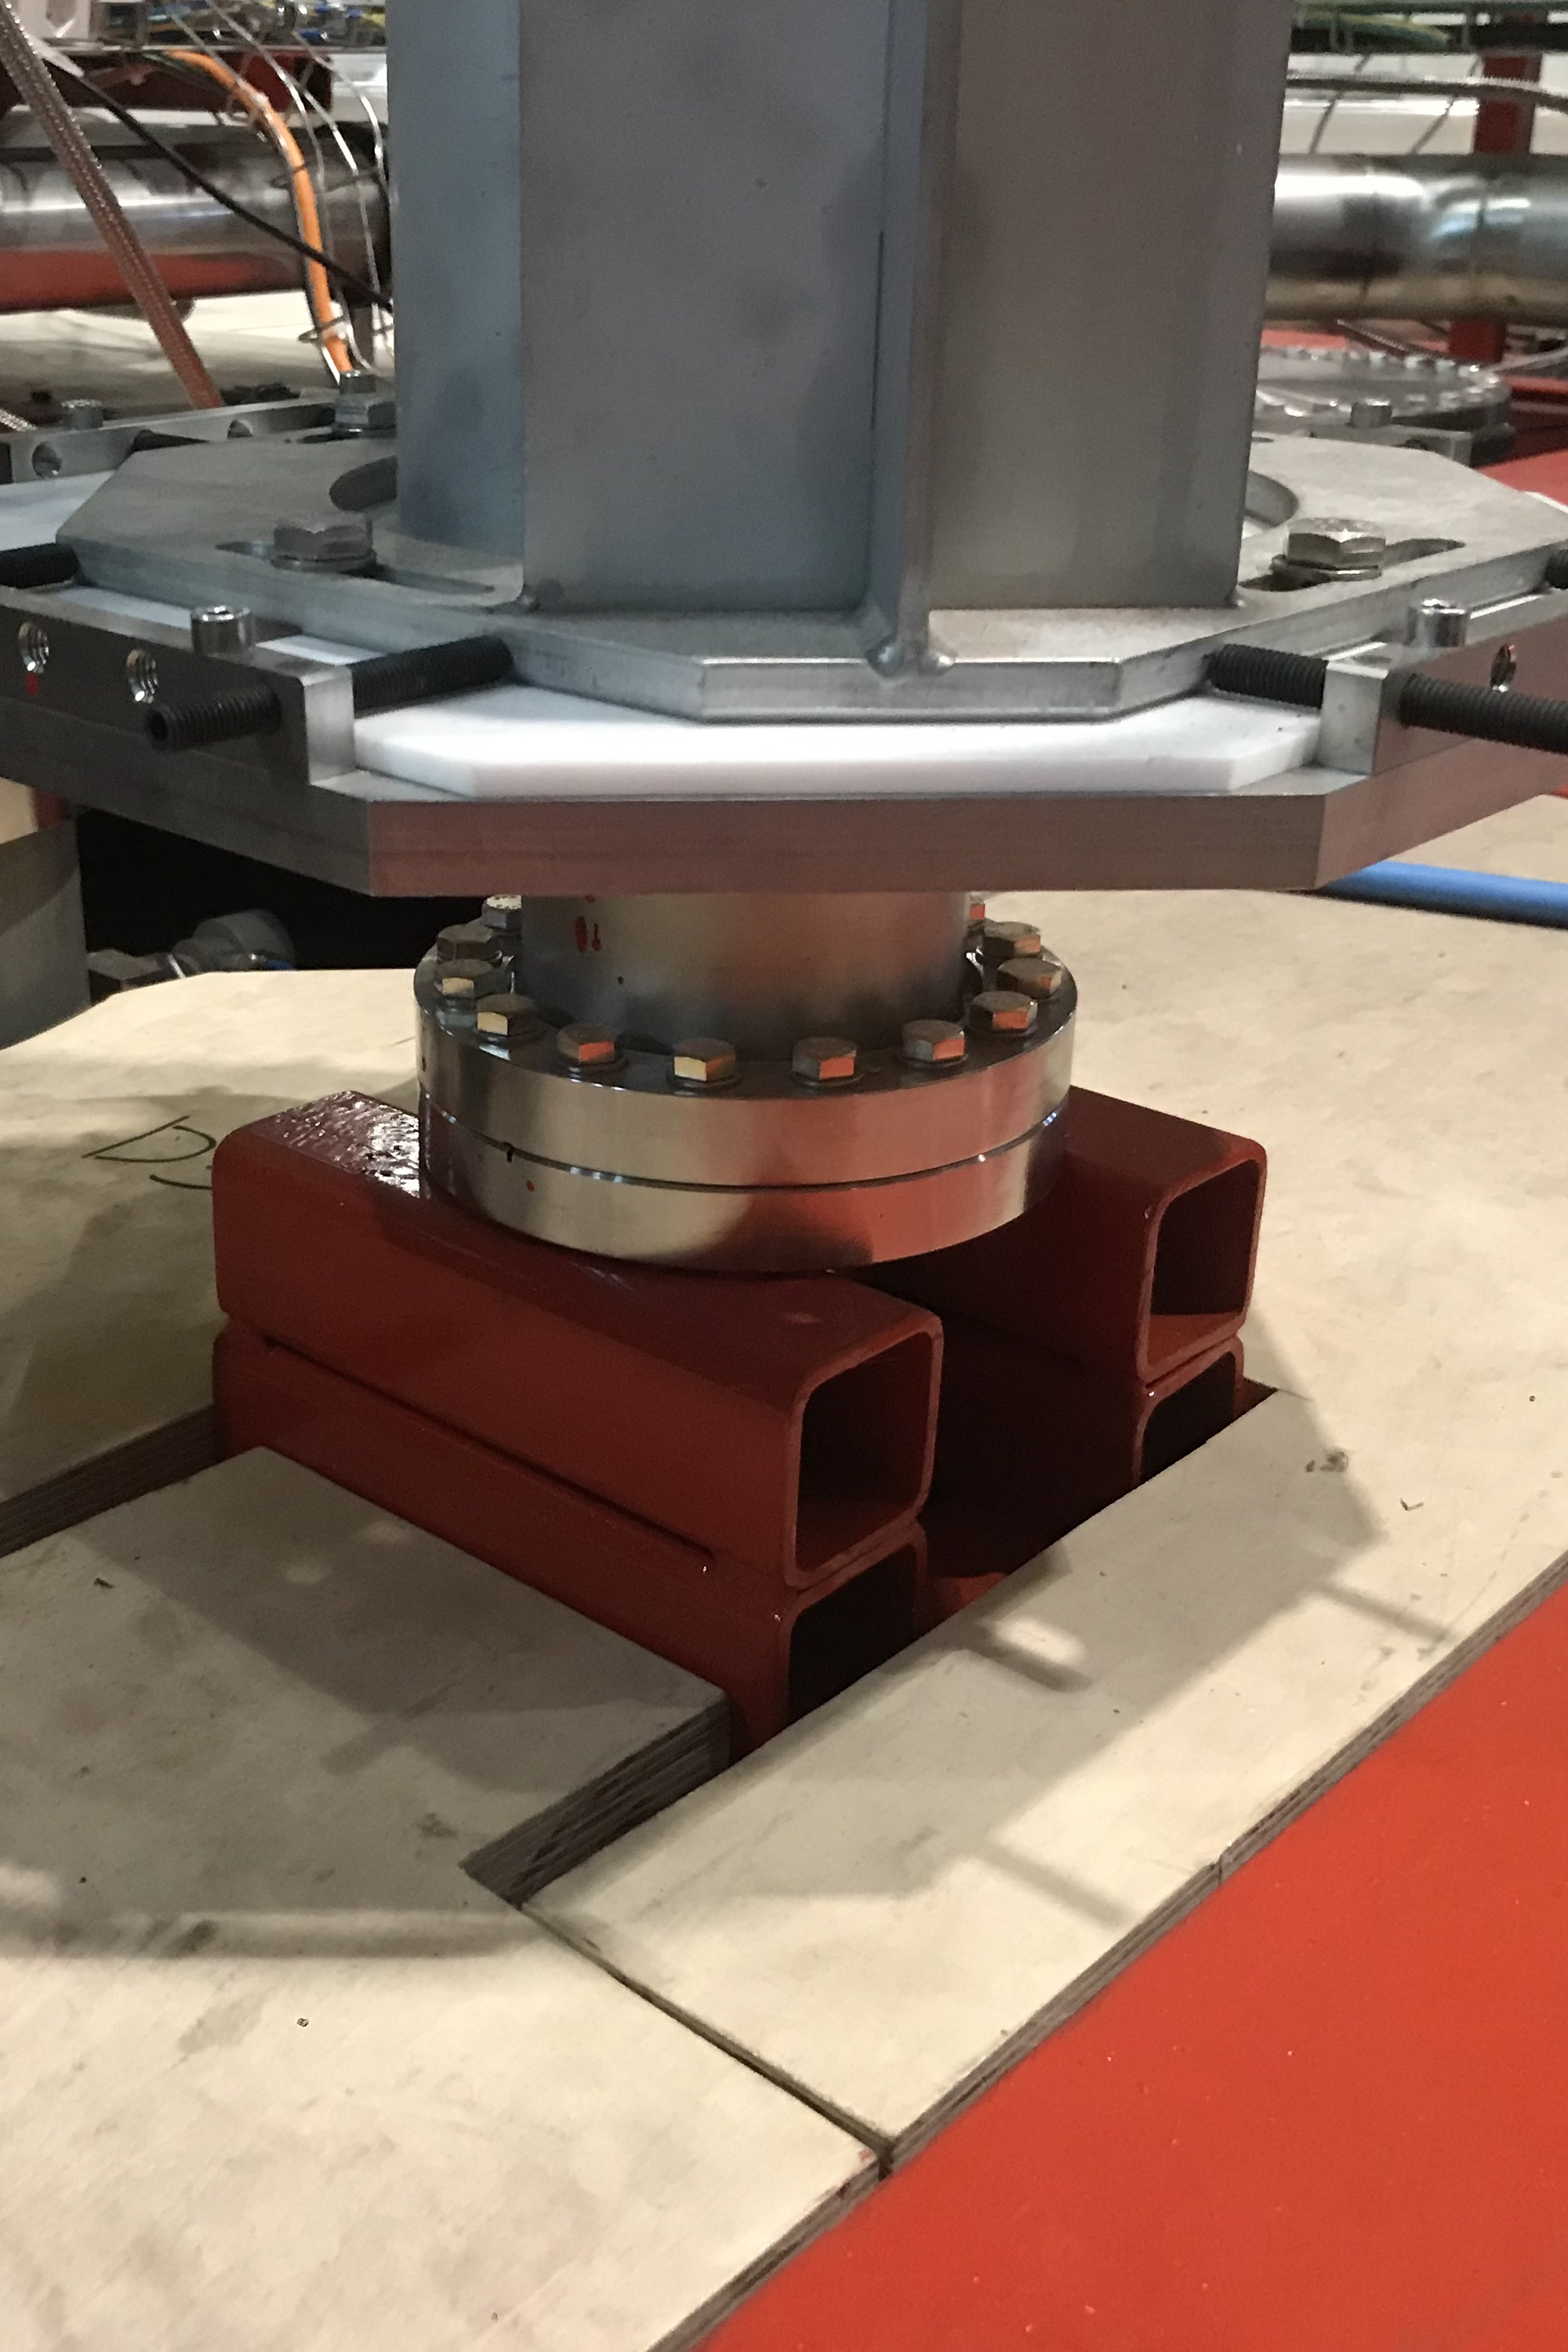
\includegraphics[width=0.45\textwidth]{crpSupport.jpg}
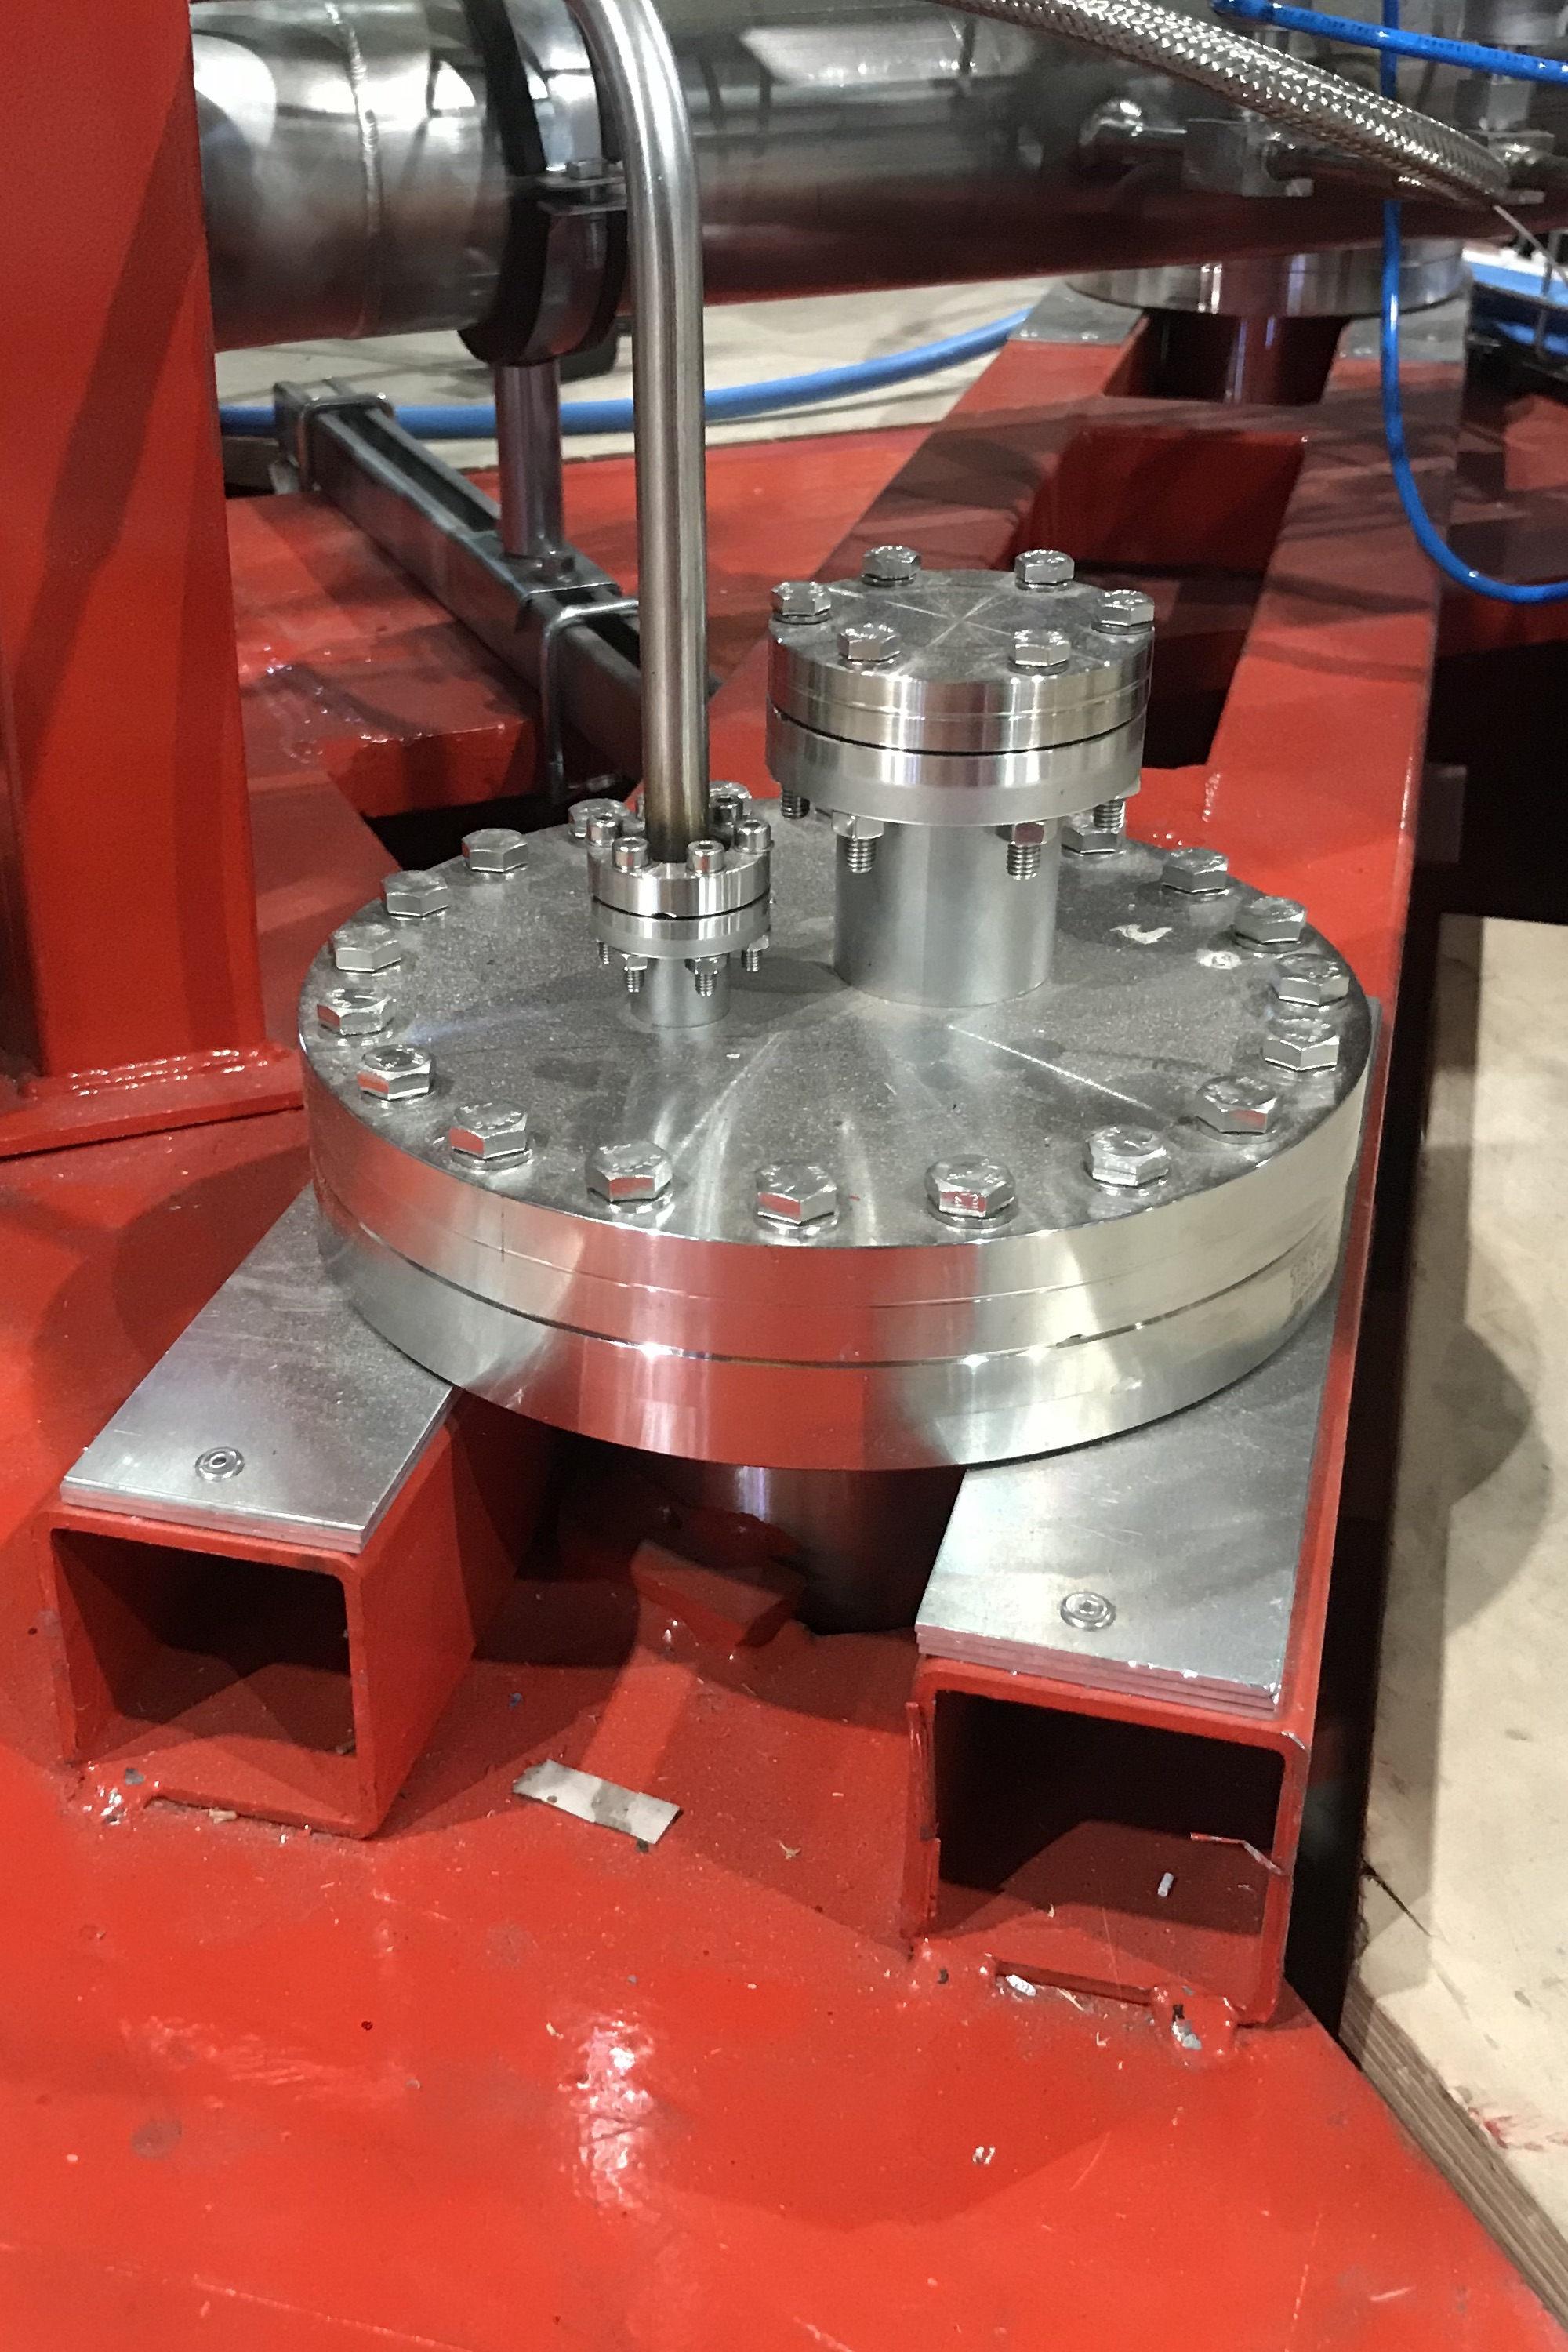
\includegraphics[width=0.45\textwidth]{fieldCageSupport.jpg}
\end{dunefigure}

All the service cables for the operation of the \dwords{crp} enters into the cryostat from what are called \dword{crp} instrumentation penetrations.
The cables passing through these penetrations are the HV for the \dword{lem} and the extraction grid, the coaxial cables for the distance meters and the level meters, the ground shielded cables for the temperature sensors, and the multi twisted pairs for the anode pulsing.
Each penetration serves two CRPs, and is positioned approximately between two adjacent \dwords{crp}.
The couple of \dwords{crp} are chosen to guarantee that during the installation sequence (from left to right in Figure~\ref{fig:DP-roof-penetration}) the penetration is always accessible by means of an elevating platform or a movable scaffold once the \dwords{crp} are in final position.
Due to the presence of the cryostat I-beams, the position of these penetrations is not symmetric with respect to the length of the cryostat.
The cabling from one of the two \dwords{crp} will be more difficult.
Internal cable trays/cable support system welded to the excess penetration tube inside of the cryostat will be used to lay the cables and guide them through the penetration releasing the mechanical stress on the connections due to the cable weight.

The field cage walls, and consequently the cathode, are attached to the roof through the field cage support penetrations.
Ten of these penetrations run along each of the long walls and two along each of the short walls.
These penetrations are used during installation: a mechanisms of pulleys the field cage is lifted from the floor inside the cryostat and lifted up to final position while actually assembling the wall.
From the same penetration the field cage will be finally hanging.
Due to the geometry of the detector and the size of the instrumented surface these penetration are unavoidably very close to the cryostat I-beam.
Along the short walls the four penetration are actually going through the I-beams, that must be therefore specially modified and consequently reinforced.
The size of the internal diameter of these penetration is large enough to allow thermal shrinkage of the field cage and cathode.

The so-called tank instrumentation penetrations are twenty openings in the roof along the cryostat long direction on both the sides.
They are meant to pass cables an instrumentation for the power and signal of the photon detectors, the optical fibers for their calibration, cable and fibers for level meters, cryogenic cameras and lighting, temperature sensors and profilers, purity monitors, and in general all the cryogenics instrumentation devices installed inside of the cryostat.
No cable trays can be connected directly to the corrugated membrane.
The cables trays can run along the internal edges of the membrane where threaded rods are welded to allow the installation of cable supports.
Dedicated cable supports and stress release devices are welded from the portion of the penetration pipe exceeding the corrugated membrane to guide the cable through penetration.
In addition, cable supports can be connected to the cryogenic pipes of the cooling sprayers to guide cables and optical fibers from the top to the bottom of the cryostat (see Figure~\ref{fig:internal-cryogenics}).

The unique \dword{hv} feedthrough penetration is located inside the surface delimited by the field cage, in correspondance of the active volume of the detector.
This design decision is due to the fact that the space between the field cage and the corrugated membrane is not sufficient to guarantee that 600~kV can be safely applied at the cathode, without the risk of electrical breakdown to ground.
The penetration is located in a corner of the \dword{tpc} underneath the detector rack mezzanine on the \dword{tco} wall.
The length of the feedthrough allows it to be inserted in the penetration when the mezzanine is in place.
The connection between the feedthrough and the cathode must go through a \dword{crp} that must therefore be special: 1~m$^2$ will not be equipped with anodes, \dwords{lem} and extraction grid.
This \dword{crp} must be installed and cabled before the connection from the \dword{hv} feedthrough and the cathode is established.

The \dword{sgft} were developed first for the 3x1x1 detector at \dword{cern} and then applied to the \dword{pddp} with a slightly different design.
Their role is to allow the electronics to be near the anode electrodes (minimize the cable lengths) and in cold (reduce the intrinsic noise of the electronics) while still having the possibility to extract the electronics without compromising the liquid argon purity.
The drawing of the \dword{sgft} used in \dword{pddp} is shown in Figure~\ref{fig:sgft-drawing}.
\begin{dunefigure}[\dshort{sgft} drawing]{fig:sgft-drawing}
{Drawing of the \dword{sgft} used in \dword{pddp}.}
\includegraphics[width=0.9\textwidth]{sgft-drawing.png}
\end{dunefigure}

The \dword{sgft} are tubes through the cryostat roof insulation.
Their inner volume is isolated form the argon and from the atmosphere.
The electronics is installed inside the tube at a level few cm below the corrugated membrane of the cryostat roof.
At the cold side of the \dword{sgft}, a flange hosts electrical connectors that connect the cables to the anode at one side and the cold electronics at the other (see Figure~\ref{fig:sgft-picture}).
A system of guiding rails along the length of the \dword{sgft} ensures that the electronics can be correctly plugged into the cold flange.
\begin{dunefigure}[\dshort{sgft} picture]{fig:sgft-picture}
{Image of the flange and the tube of the \dword{sgft} used in \dword{pddp} prior assembly.}
\includegraphics[width=.5\textwidth]{sgft-picture.jpg}
\end{dunefigure}
This flange is crucial because at cold it isolates the ultra-pure argon.
The \dword{sgft} volume is filled with nitrogen or argon to avoid moisture condensation on the electronics.
The temperature at the bottom of the \dword{sgft} is not low enough to allow the condensation of argon.
Having argon at 1~bar as the atmosphere inside the \dwords{sgft} would reduce the possible \dword{lar} contamination consequent to the development of a leak in the cold flange.
Each \dword{sgft} before installation must be electrically tested and helium leak must be proven to be better than $10^{-8}$~mbar$\times$L/s at room temperature.
At least the cold flanges must be leak tested at cryogenic conditions too.

%DESCRIPTION OF THE LAYOUT OF THE CABLE TRAYS. NOT YET FULLY DEFINED.

%DESCRIPTION OF THE LAYOUT OF THE ELECTRONICS RACKS. NOT YET FULY DEFINED.

%BRIEF DESCRIPTION OF THE PURGE PIPES. SCOPE OF THE CRYOGENICS.

\subsection{Cryostat Interior}
The internal cryogenics comprises manifold of pipes to ensure the proper detector purge, cool-down, filling and re-circulation of \dword{lar}.
A 3D view of the inside of the \dword{dpmod} with the cryogenic pipes is shown in Figure~\ref{fig:internal-cryogenics}
All pipes enter the cryostat from the cryo penetrations on the roof.
The \dword{gar} distribution system consists of a set of pipes installed on the cryostat floor (shown in red in Figure~\ref{fig:internal-cryogenics}).
These pipes are used only prior to filling to remove the air in the cryostat.
They have either a longitudinal slit or calibrated holes to distribute \dword{gar} uniformly along the length of the cryostat.
The piston purge effect was successfully tested in \dword{pdsp} and  \dword{pddp}.
In order to efficiently extract the air, turbulence must be avoided while purging with warm \dword{gar}.
The optimal filling speed is estimated to be 1.2~m/h (vertical height in the cryostat).
\begin{dunefigure}[Internal cryogenic piping]{fig:internal-cryogenics}
{3D model view of the internal cryogenic piping.}
\includegraphics[width=0.9\textwidth]{internal-cryogenics.png}
\end{dunefigure}

The \dword{lar} distribution system consists of a set of pipes again installed on the floor of the cryostat (shown in blue in Figure~\ref{fig:internal-cryogenics}).
They are required for flowing \dword{lar} over a broad range of flow rates.
These pipes are used to fill the cryostat and, during steady state operations, to return the \dword{lar} from the purification system.
These pipes have calibrated holes to return the LAr uniformly throughout the length of the cryostat.
This is fundamental to maintain uniform purity along the full length of the detector.
Four pumps circulate the \dword{lar} inside the cryostat, all of which operate initially to achieve the desired purity.
Once the target purity is achieved, only one or two pumps remain in service.

A system of \cooldown sprayers is installed along the two long walls of the cryostat just below the ceiling.
One set distributes \dword{lar} using liquid sprayers that generate a conical profile of small droplets of liquid.
The other set of sprayers distributes \dword{gar} to move the \dword{lar} droplets inside and cool down the detector and cryostat uniformly.
These sprayers are being tested in \dword{pddp} and are a modified version of the ones used in \dword{pdsp}.
The cooling system design for \dword{dune} is being updated while this chapter is written, therefore the solution that will actually be implemented may differ from what described above.


Other infrastructure inside the cryostat includes the cryostat false floor, the UV-filtered lighting, and the battery-operated scissor lifts.
The false floor must ensure a flat surface above the internal cryogenic pipes to allow the safe operation of the man lift and the positioning of the scaffold.
The heaviest load that the false floor must support is the 14~m high man lift, though the requirements for the false floor are not yet fully defined.
Following the experience of \dwords{protodune} the false floor can be made out of plywood panels fixed on wood blocks that defined the false floor height.
The wood blocks are simply standing on the flat part of the corrugated membrane, with some plastic protection to avoid damage to the corrugated membrane.
The wood must be painted to minimize wood dust in the cryostat and it must also be treated with fire retardant agents.
The floor must be composed of sections that can be independently and easily dismounted according to the needs of the installation.
This is fundamental when installing the \dword{pd} and the ground grid, since they occupy the space taken by the false floor.

The cryostat lighting, using UV-filtered LED lamps, is expected to be fairly simple.
Floor-mounted lights and lights entering from some roof penetrations will be investigated.
Options for the lighting will be developed further.

At least one commercially-available battery-operated scissor lift with a 14~m reach is used to work on the \dword{crp} installation and cabling as well as for the installation of the field cage and the cryogenics instrumentation.
Tests at Ash River will verify the stability of the lift at height.
If the lift is determined to be suitable, then the remaining issue to resolve is how to insert and remove it from the cryostat.
Commercially-available scissor lifts are too wide to fit easily through the \dword{tco} opening where one of the large cryostat support I-beams protrudes above the floor level.
Custom lifting equipment is needed to insert and remove the lifts into the cryostat.
The cavern overhead crane in conjunction with the cleanroom crane (see next section) can be used to transport the most heavy objects in and out of the cryostat.
At the end of the installation process, the last lift may require partial dismantling before it can be removed from the cryostat.

\subsection{Cleanroom}
The underground cleanroom in front of the \dword{tco} is the main place where the detector components are unpacked, assembled and tested prior the installation inside the cryostat.
The experience in building \dword{pdsp} and \dword{pddp} showed that the role of the cleanroom is fundamental in several aspects.
The cleanliness of the air and the absence of powder and dust is fundamental for all the detector components, and in particular for the \dwords{lem} in the \dwords{crp}.
The cleanroom should ensure the adequate cleanliness of the air where the detector components are unpacked and tested, and it should meet ISO-8 cleanroom class standards.
The cleanroom also isolates and protects the inside of the cryostat from the dirty environment of the cavern, which has exposed exposed rocks and non-protected floor.
In order to achieve this, a properly sized ventilation and air filtration system is required.
The requirements for work in an ISO-8 cleanroom are a cleanroom lab coat, clean shoes, or shoe-covers, and nets for hair and beards.
This is in addition to a clean hard hat and gloves for safety reasons.

The cleanroom must provide space and tools to test the detector equipment, most notably the \dwords{crp} in the  \coldbox{}es and the \dword{pmt} tests in the dark box.
Compared to the \dword{spmod} the cleanroom is smaller in all  directions, since most components do not need to be assembled prior installation, and the major assembly work of the cathode and field cage is done directly inside of the cryostat.

Two views of the \threed model of the cleanroom are shown in Figure~\ref{fig:cleanroom}.
The cleanroom surrounds and seals against the \dword{tco} to isolate the cryostat.
The \dword{tco} can be temporary closed with plastic curtains, to isolate the cryostat from possible dirty jobs inside the cleanroom.
The tallest component to enter the \dword{tco} is the \dword{crp} box which is a 3.2~m.
The \dword{tco} is therefore smaller compared to the \dword{spmod}.
The opening is about 2.6~m large and 5.2~m tall, that is sufficient pass the \dword{crp} box with the slings and lifting tool.
The small size of the \dword{tco} permits that its closure can be done once the \dword{tpc}, and in particular the \dword{fc} are fully mounted.
The \dword{tco} that is shown in Figure~\ref{fig:cleanroom} is only for visually representing the opening dimensions.
The actual engineering of this part will be detailed in the future, before the beginning of the 2021 when the final cryostat model of the \dword{pddp} will be available.

The mechanical structure for the cleanroom is a self sustained steel skeleton where the walls, made out of rigid aluminium-foam-aluminium sandwich panels, are fixed.
The size of the cleanroom are about $16 \mathrm{(L)} \times 16 \mathrm{(L)} \times 9 \mathrm{(H)}$~m$^3$.
The floor must be covered with resin or other material that is simple to keep clean.
The cleanroom floor and the objects inside the cleanroom must undergo regular cleaning in order to ensure all the time the ISO-8 class standard.

\begin{dunefigure}[Internal cryogenic piping]{fig:cleanroom}
{Two views of the 3D model of the cleanroom in front of the \dword{tco}.}
\includegraphics[width=0.9\textwidth]{cleanroom1.png}
\includegraphics[width=0.9\textwidth]{cleanroom2.png}
\end{dunefigure}

The cleanroom layout can be seen in Figure~\ref{fig:cleanroom} (bottom).
Around the \dword{tco} enough space is left in order to install and access the four liquid argon pumps that stay on the cryostat level on the two sides of the \dword{tco}.
The cleanroom is equipped with four  \coldbox{}es, overhead mobile cranes, a material airlock, a personnel airlock, space for the cryogenics to operate the  \coldbox{}es, and a room to test the \dwords{pmt} in a dark box.
Additional space may be required to work on detector components that need to be modified/fixed/refurbished and for which the work does not justify to bring the component on surface.
An additional $5\times6$~m$^2$ equipped with two gantry cranes to lift one \dword{crp} may be needed.
The material airlock is large enough to house one \dword{crp} box; that is the widest component that needs to enter.
The material access is done at the cryostat level through two 3.8~m large rolling doors.
Unlike \dword{pdsp} and \dword{pddp}, in this case the airlock does not need to have an openable roof.
Nonetheless, this option can be easily implemented in the present design of the cleanroom.
In this airlock the material is cleaned and if needed unpacked before entering into the actual cleanroom.
For the components that are longer than the length of the airlock, as the I beam that support the filed cage, both the doors can be temporary and shortly opened to allow the access of the material without compromise the quality of the air in the cleanroom.
In case of longer operation that require both rolling doors to be opened, temporary plastic curtains can be installed to limit the powder and dust from the cavern to enter into the cleanroom.
The airlock is large enough so that a standard fork-lift can enter and maneuver.
Inside the cleanroom, instead, due to space constraints only manual forklift can be used.

The cleanroom hosts four \coldbox{}es and the cryogenics infrastructure in order to operate them.
The  \coldbox{}es are arranged in two rows along the walls of the cleanroom, one in front of the other.
The central region is used to manipulate the \dword{crp} box and to attach the \dword{crp} below the  \coldbox roof.
This region is also used to manipulate all the elements prior insertion in the cryostat.

The cryogenics for the \coldbox{}es is not fully defined and detailed yet.
The tall cryostats shown in Figure~\ref{fig:cleanroom} are mostly a place-holder.
If more space is required for the cryogenics installation, the area outside the cleanroom can be used, since the cryogenics does not need to be installed in a clean environment.

Along the width of the cleanroom and above the \coldbox{}es there are I-beams equipped with trolleys and electrical hoists that serve as 2~ton over-head cranes to open and close the  \coldbox{}es.
These I beams may be connected to the cavern walls or the steel structure of the cleanroom.
A third I-beam connects the \dword{tco} structure to the cleanroom structure and in the same way it is used as crane to bring material inside the cryostat.
The heaviest detector component to be brought inside the cryostat is the \dword{crp} in its box.
Its total weight is below 800~kg.
No major activities at height are needed inside the cleanroom.
For the lifting of the \dword{crp} box and in order to insert it inside the cryostat there will be available at least one 8~m-tall compact man lift, which can be seen parked in two positions inside the cleanroom in Figure~\ref{fig:cleanroom}.

The \dword{crp} in its box is not the heaviest object to enter into the cryostat.
In fact, despite not having yet identified the 14~m tall man lift, it will certainly be heavier (order of 3~tons).
A custom tool to insert heavy object inside the cryostat must be developed and possibly to be used in conjunction to the cavern crane and the cleanroom crane.
For this reason, the cleanroom roof in front of the \dword{tco} and the I-beam that enters into the cryostat can be removed.
This operation will be necessary also to complete the closure of the external structure of the \dword{tco}.

\subsection{ \Coldbox{}es}
An electrical and mechanical test of each entire \dword{crp} in realistic cryogenic thermodynamic conditions and in reasonably pure argon vapor must be performed in order to access the final \dword{qc} of the \dword{lem} and \dword{crp} assembly before the installation in the cryostat.

The tests are performed in four dedicated cryostats, also referred to as \coldbox{}es, installed in the cleanroom in front of the \dword{tco} and with dedicated cryogenics infrastructure that allows to operate each of them independently.
The objectives of the global test of the \dwords{crp} are:
\begin{itemize}
\item the characterization of the \dword{hv} operation of each \dword{lem} independently and as well the \dword{hv} operation of all the 36~\dwords{lem} forming a \dword{crp} at the same time,
\item the characterization of the \dword{hv} operation of the extraction grid,
\item the test of all the \dword{hv} contacts from the feedthroughs to the \dword{lem} and grid connectors,
\item the measurement of the flatness of the \dword{crp} during the test and the capability to align the \dword{crp} to the \dword{lar} level, and 
\item calibration of the level measurement from the capacitance between the extraction grid and the bottom electrode of the \dword{lem}.
\end{itemize}

The requirements for the environment of this test are defined as follows:
\begin{itemize}
\item The \dword{lar} surface must be flat within 2~mm in order to allow the \dword{lem} to be in the vapor phase and the grid in liquid phase.
\item The vapor pressure does not need to be stabilized, but it must constantly be monitored.
\item The vapor temperature should not be controlled, but constantly monitored.
\item The liquid argon purity should be of the order of at most 100~ppm (O$_2$ equivalent), in order to be comparable with the tests at 3.3~bar and room temperature done for each \dword{lem} during the \dwords{qc} before reaching \surf.
\item The \dword{crp} vertical position and horizontality should be adjustable, at least before the filling of the  \coldbox.
\end{itemize}

Figure~\ref{fig:NP02-ColdBoxSketch} shows a sketch of the  \coldbox.
The same concept of  \coldbox was successfully used several times at \dword{cern} in 2018 to characterize the four \dwords{crp} installed in \dword{pddp}.
\begin{dunefigure}[Sketch of the \coldbox]{fig:NP02-ColdBoxSketch}
{Schematic representation of one \coldbox for the test of the \dwords{crp}.}
\includegraphics[width=0.9\textwidth]{NP02-ColdBoxSketch.png}
\end{dunefigure}
The external structure is a self-supporting box made out of 1~cm-thick stainless steel plates.
The internal membrane is made out of 2~mm-thick stainless steel plates.
The internal dimensions are 1~m in height and 3.9~m in the other directions.
The thermal insulation is passive and it consists of four layers each of 10~cm-thick polyurethane foam (30~kg/m$^3$).
The insulation layers are separated by polyethylene foils to minimize the convection phenomena and the consequent increase of heat input.
The insulation region is flushed with  nitrogen gas, as is done for all the corrugated membrane cryostats.
The  \coldbox{}es are too large to be transported underground, therefore they must be produced in place during the construction of the cleanroom.
A custom made RGA-based dense gas analyser monitors the composition of the gas nitrogen circulating in the insulation space.
The same system may be used to monitor the quality of argon boil-off with a sensitivity of about 50~ppm of O$_2$ and N$_2$.

The \dwords{crp} are attached to a portion of the roof (shown in blue in Figure~\ref{fig:NP02-ColdBoxSketch}) that can be opened.
The horizontality and the vertical position of the \dword{crp} can be adjusted within about $\pm 20$~mm around the nominal position.
The adjustment is done manually from the hanging system installed on the  \coldbox roof very similar to the one finally used in the cryostat.

The liquid argon level in the  \coldbox is kept constant by compensating the losses due to the evaporation with new liquid argon.
The cold boil-off vapor is sent to the cryogenics systems via vacuum insulated pipes to be re-condensed in a closed loop cycle.
The cryogenics system, that is not yet detailed, should cope independently with the four  \coldbox{}es, in order to allow maximally flexibility during operation.
The cryogenics system should be able to cool-down one  \coldbox equipped with the \dword{crp} and fill it with the liquid argon in at most two days.
The same time is allocated to empty the \coldbox, warm it up, and purge the volume with breathable air.
In order to empty the  \coldbox once the test is concluded, a 10~kW heater is used to evaporate the liquid argon, which is then re-condensed by the cryogenics system and stored in a standard vacuum insulated cryostat.
The storage should be able to contain at least the liquid argon from all the four  \coldbox{}es.
It is not expected to empty more than one  \coldbox at a time, therefore the heat budget that the cryogenics system must cope with is the heat loss of the  \coldbox{}es (rounded at 4~kW), the inefficiencies of the transfer lines (that depends on the design), the inefficiencies of the cryogenics system and the condenser, and the heater to empty the boxes.
It is possible, instead, that while emptying one  \coldbox, another one is filled.
The cooling of the  \coldbox and the \dword{crp} introduce additional charge on the cryogenics system.
No purification circuit is require in order to obtain a liquid argon contamination compatible with drifting electrons.
Part per million contamination is required in the gaseous argon.
Since the  \coldbox{}es are often opened, it is probable that to guarantee the needed purity some sort of purification cartridge on the argon circuit must be installed.
In case of loss of argon during the ten months of operation of the  \coldbox{}es, the cryogenics system should be design in such a way that more argon can be taken from the surface.

The operation of the \dword{pddp}  \coldbox proved that the requirements can be met and exceeded.
Figure~\ref{fig:NP02-cold-box} shows the \dword{pddp}  \coldbox prior being closed for a test.
A \dwords{crp} is hanging from the roof and it is being closed inside the box.
\begin{dunefigure}[Photo of the \dshort{pddp} \coldbox]{fig:NP02-cold-box}
{Photo of the \dword{pddp} \coldbox open and with a \dwords{crp} hanging from the roof.}
\includegraphics[width=0.9\textwidth]{NP02-cold-box.jpg}
\end{dunefigure}

During the tests, the contamination of nitrogen and oxygen was always well below 100~ppm and the measurement was limited by the sensitivity of the instrument.
The level was monitored with a coaxial capacitive level meter and it was also monitored by means of eight capacitive level meter installed around the \dword{crp} with a precision of 250~$\mu$m.
The level was automatically and constantly adjusted to the nominal value refiling the  \coldbox with new liquid argon.
The liquid argon evaporation resulted in a level decrease of about 0.7~mm/h\footnote{The evaporation rate is a simple method to evaluate the heat input due to the  \coldbox only which results in less than 700~W. In the case of the \dword{pddp}  \coldbox, the argon was let evaporate and replaced with new argon to maintain the level.}.
A simplified version of the \dword{pddp} final suspension system allows adjustment of the position of the CRP with respect to the liquid argon level using three manual winches changing the height of the CRP at the level of the anchoring points in steps of 0.4~mm.
To complete the  \coldbox instrumentation, three cryogenic cameras were used to monitor the \dword{crp} from below and above.
One camera was positioned to give a side view of the \dword{crp} with a field of view of the order of 40~cm.
In Figure~\ref{fig:NP02-ColdBoxCamera} one can appreciate the flatness of the liquid argon level, which is much better than 2~mm even when the regulation of the liquid argon level is functioning.
\begin{dunefigure}[Image from inside the \dshort{pddp} \coldbox]{fig:NP02-ColdBoxCamera}
{Photo from the inside of the \dword{pddp} \coldbox at \dword{cern} during a \dword{crp} test.}
\includegraphics[width=0.9\textwidth]{NP02-ColdBoxCamera.jpg}
\end{dunefigure}




%\cleardoublepage

\section{Detector installation}
\label{ch:dp-tc-installation}

The detector installation starts once the cryostat and the internal cryogenic piping is completed.
A false floor capable of holding the weight of a 14~m reach man-lift or a movable scaffold is available.
The ISO-8 clean room next to the cryostat equipped with four cold boxes and the related cryogenic must also be completed and functional.

The \dword{dp} detector is a single active volume device with the \dwords{crp} plane parallel to and at the level of the liquid argon surface, the field cage walls installed vertically to delimit the active volume, the cathode plane hanging from the field cage at the bottom.
The photo-detectors are installed below the cathode, and they are protected from the strong electric field by a ground grid that covers them.
The \dword{dpmod} is completed with a set of cryogenic instrumentation devices that permits the proper operation of the detector.
The cold electronics for the charge readout is installed on the roof of the cryostat.
A number of additional items, like the safety control system, detector control system, \dword{daq} racks complement the detector.

The access to insert large detector components into the cryostat is the \dword{tco}, a large opening in one of the two short walls of the cryostat.
Given the structure of the \dword{tpc}, the installation starts from the opposite side of the \dword{tco}.
The \dwords{crp}, the field cage, and the cathode hang from the cryostat roof.
The natural installation of the \dword{tpc} is in sections and according to the following sequence: the cryogenic instrumentation far from the \dword{tco} wall is installed first,
the field cage and \dwords{crp} - that is the most time consuming installation activity - follow, the cathode sections are the next, and the \dwords{pmt} and the ground grids complete the sequence.

The installation of the entire \dword{dpmod} is driven by the rhythm of testing and installation of the \dwords{crp}.
The installations of the \dwords{crp} and the field cage are mostly independent.
Nonetheless, due to space constraints and access requirements around the \dwords{crp} at height, the installation at the same time of a portion of the field cage and the \dwords{crp} next to it is not possible.

At least a two-people scissor-lift capable of reaching the ceiling from the false floor in the cryostat is the ideal means to work at height.
The main advantage is the ability to move easily and quickly.
This would make the work more flexible and efficient in case of installation conflict due to problems or unforeseen issues.
This lift has not yet been identified.
The typical dimensions of typical lift are 2.5~m in height when stowed and 1.2~m in width.
Lift that can extend the platform at about 12~m (14~m reach) and weight at least 3~ton typically do not need extension feet.
Several of this kind are available on the market.
Scaffold is also considered as an option.
Due to the limited space, scaffold may be the only solution to reach the ceiling between the field cage and the cryostat membrane.
The advantage of scaffold is that it is more stable compared to the scissor lift, and more than two people can work at eight at the same time.
Obviously, scaffolds are more difficult to move and therefore the installation procedure can be less adaptive to follow unforeseen events.

\begin{dunefigure}[Global installation sequence]{fig:globalInstallationSequence}
{Global installation sequence.}
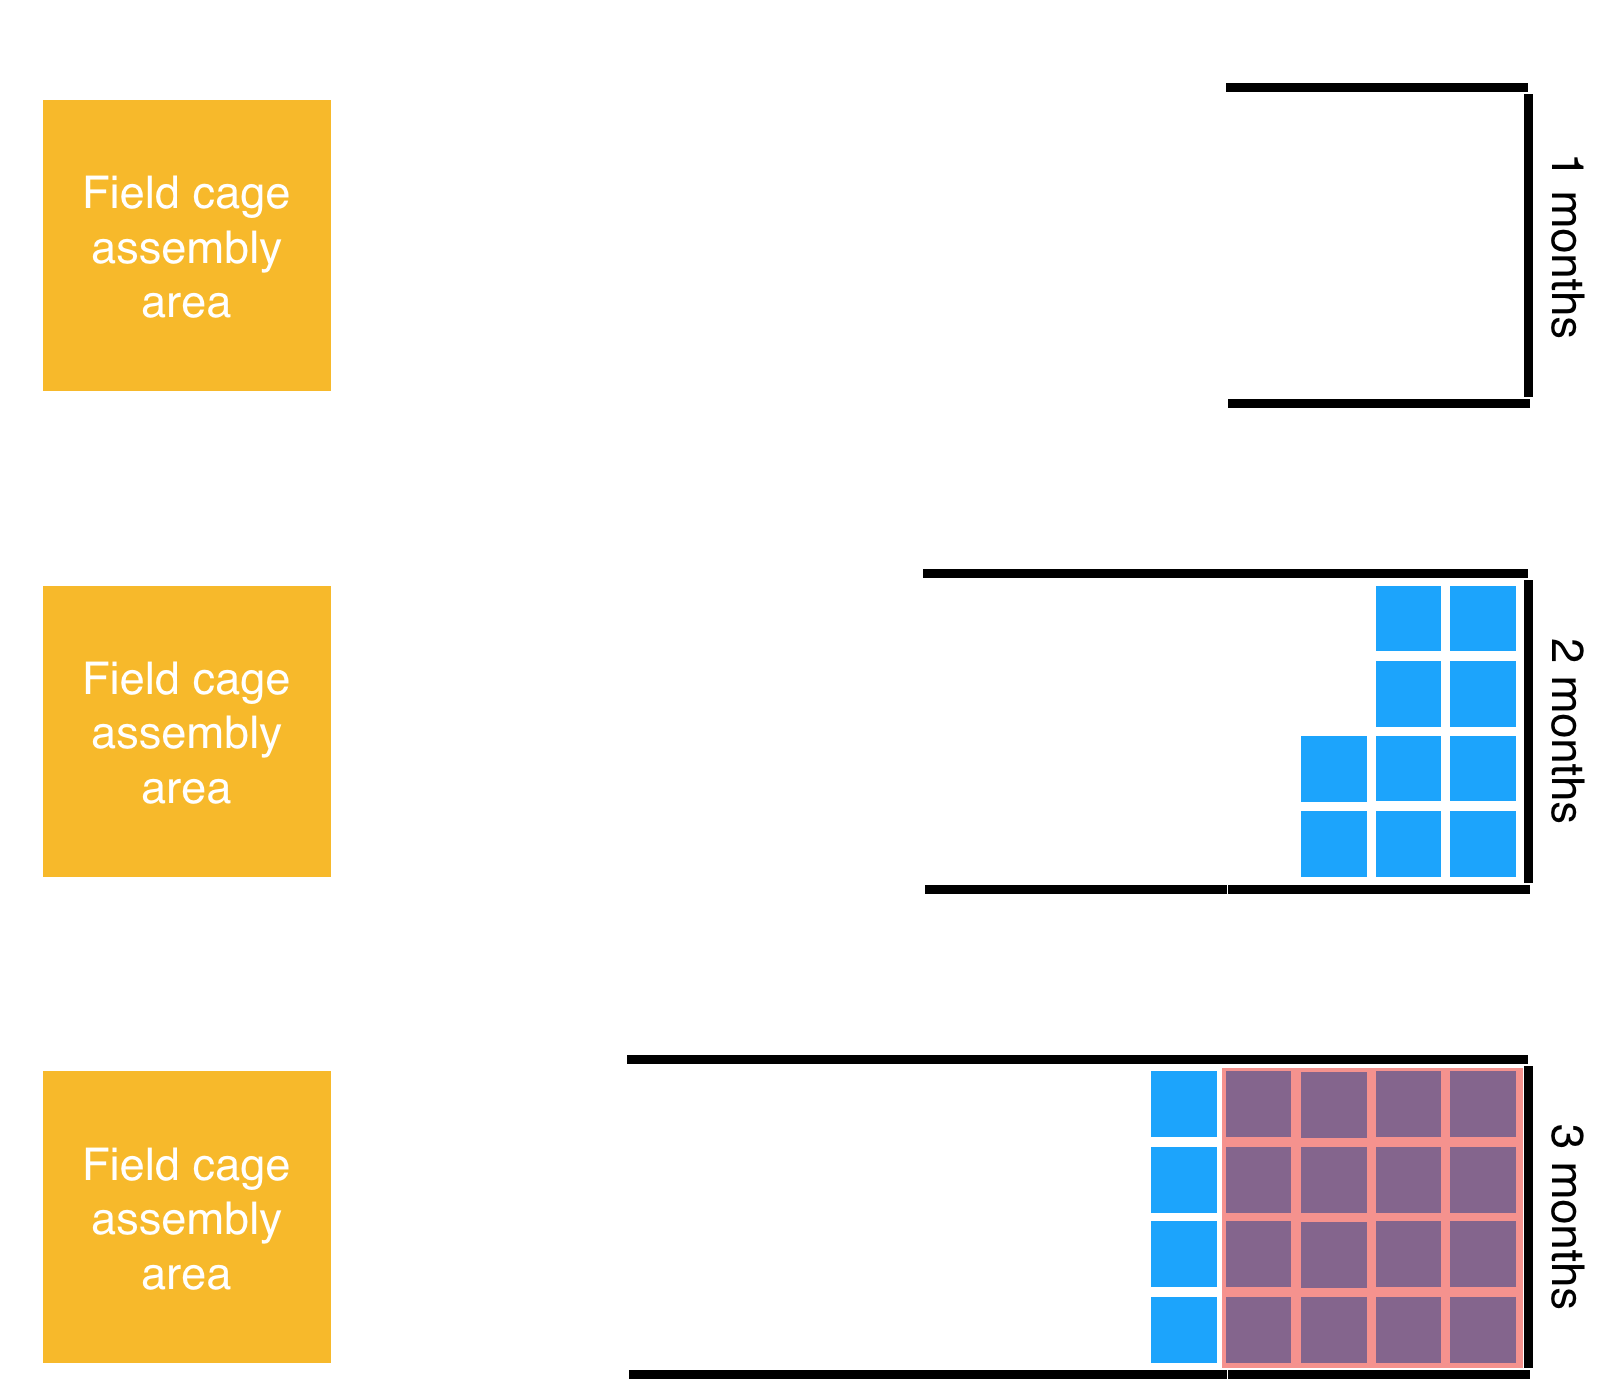
\includegraphics[width=0.5\textwidth]{installationSequence1.png}
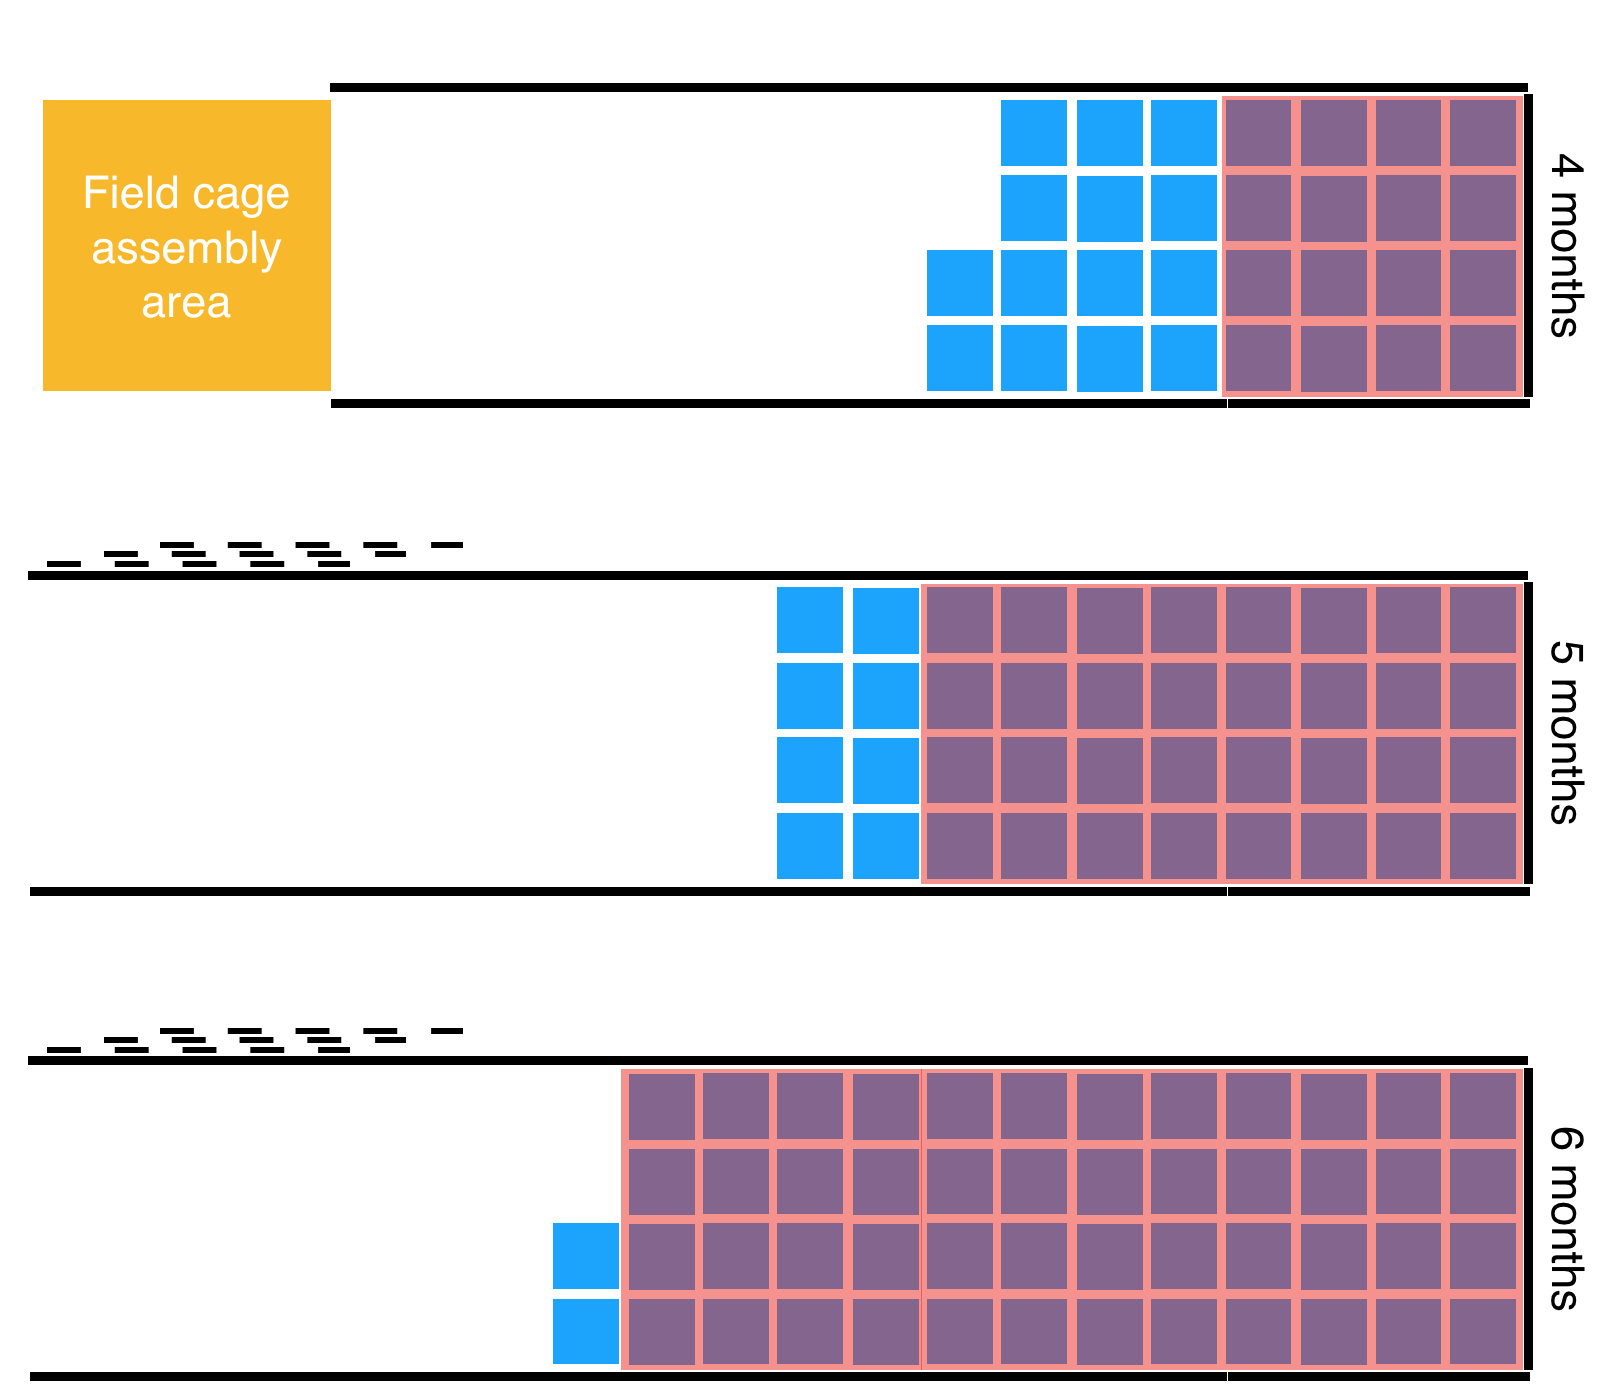
\includegraphics[width=0.5\textwidth]{installationSequence2.png}
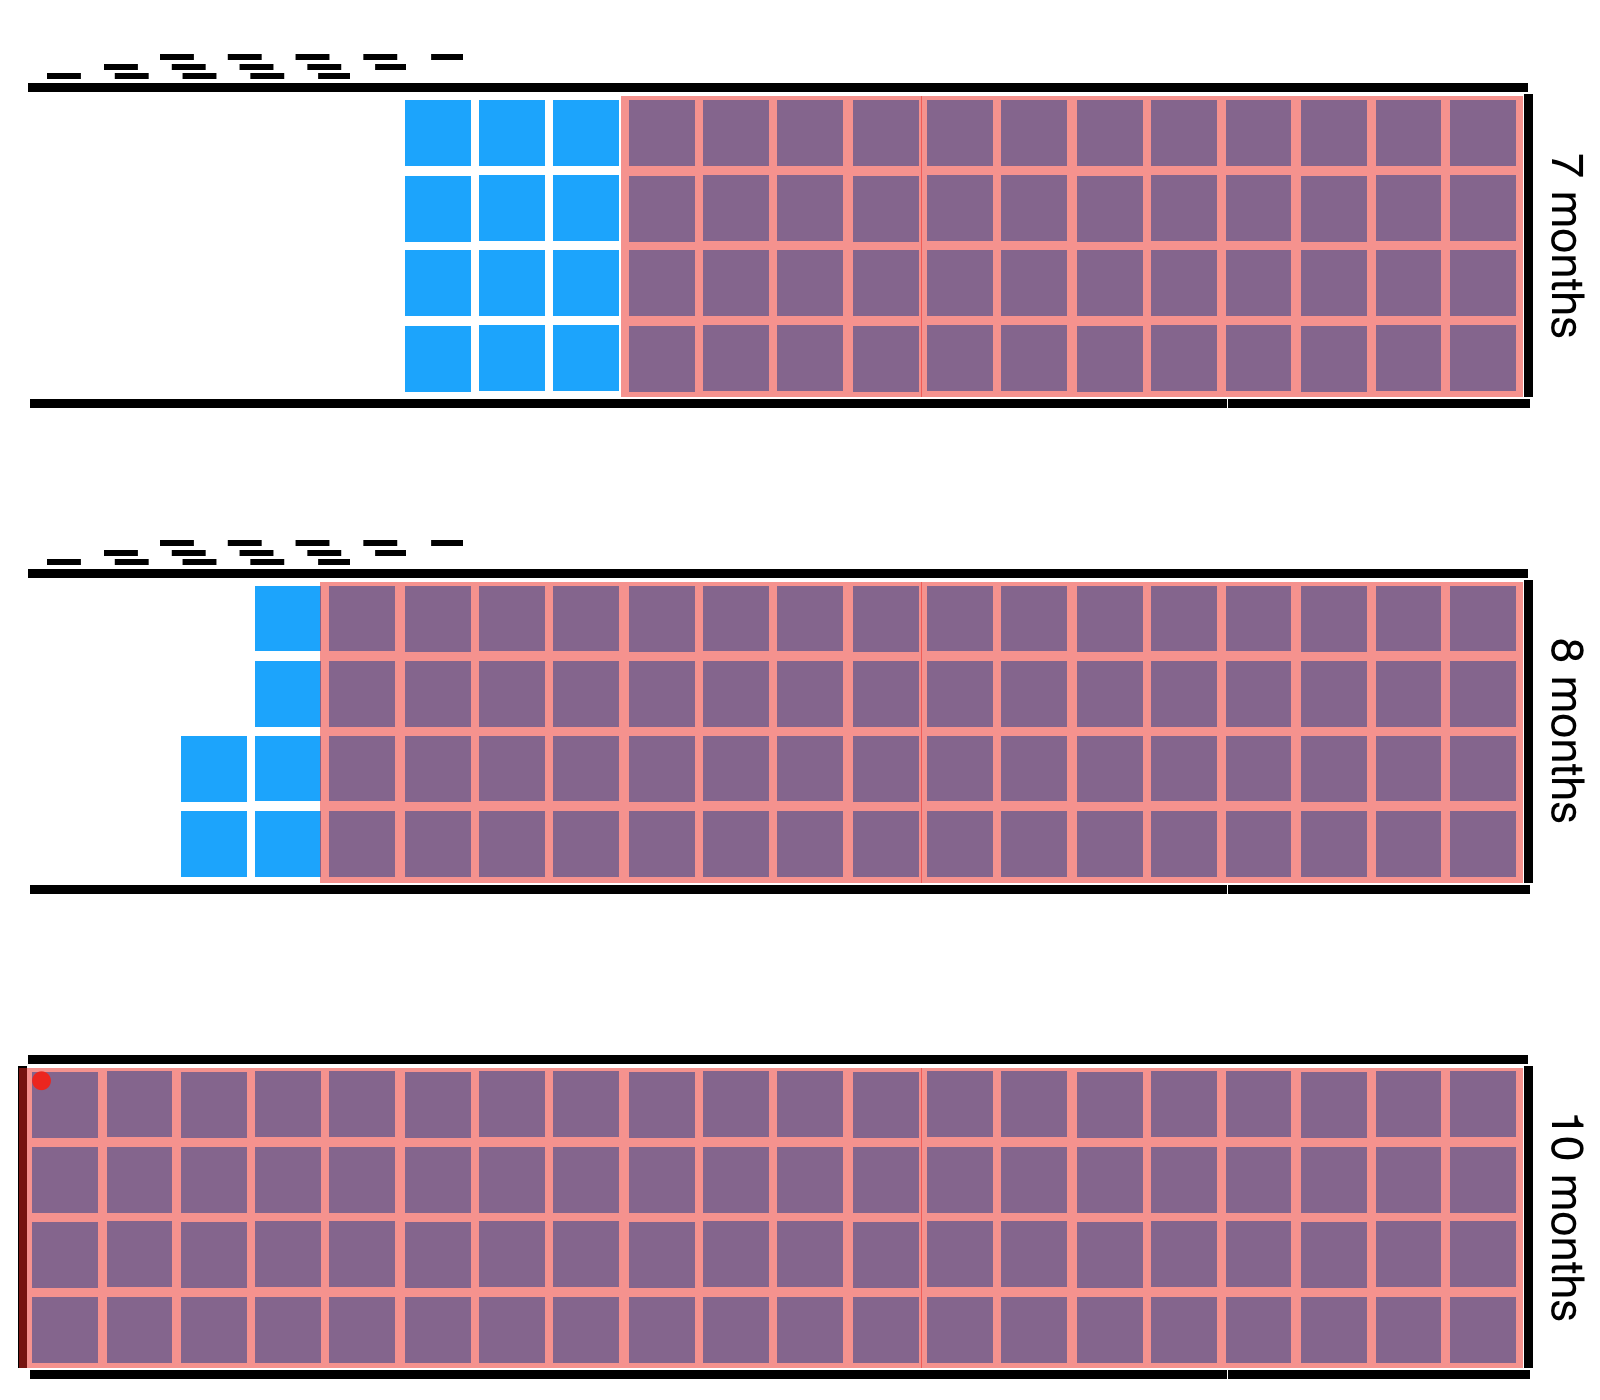
\includegraphics[width=0.5\textwidth]{installationSequence3.png}
\end{dunefigure}

Figure~\ref{fig:globalInstallationSequence} shows the global and overall sequence of installation of the \dword{dp} \dword{tpc}.
The \dword{tco} is on the left side of this sketch.
The orange area is dedicated to the assembly of the \dword{fc}.
This zone is large enough to allow confortably the assembly and the storage of the \dword{hv} system components and the access of material and personnel to the cryostat through the \dword{tco}.
This zone is temporary, and it will be use for the first four months of activities inside the cryostat.
At that time, all the field cage installation will be completed except for the end-wall in front of the \dword{tco}.
The \dword{fc} sub-modules, nonetheless, will be assembled and ready to be installed when needed.
The \dword{fc} installation preceeds always the \dword{crp} installation except for the end-wall on the \dword{tco} side.
The \dwords{crp} are installed at rate of ten \dwords{crp} per month.
The rhythm is dictated more by the cold box tests other than the actual time it takes the to install the \dwords{crp}.
The connection of all the \dword{crp} related cables is the most time consuming and delicate activity.
The finalisation of the \dword{crp} \dword{hv} connection may need extensive work on the cryostat roof, if it is done in the same way as \dword{pddp}.
At roughly the same installation rate, the cathode, the ground grid and the \dwords{pd} are installed.
In this case, the most assembly of the cathode will drive the activities inside the cryostat.
Once the cathode is installed, the ground grids and the \dwords{pmt} installation will flawlessly keep the pace.
The last two busy months of \dword{tpc} installation are dedicated to the completion of the \dword{crp} installation, assembly and installation of the last \dword{fc} end-wall, installation of the cathode, ground grids and \dword{pmt} and the installation of the \dword{hv} extender to connect the \dword{hv} feedthrough to the cathode.


\subsection{Charge readout plane installation}
The \dwords{crp} are transported in a box that make the \dword{crp} assembly a more solid structure, it protects the fragile devices in the \dword{crp}, like the extraction wires, and it keeps it clean.
The size of the transportation boxes is $3.2\times3.5\times0.8$~m$^3$ and it is compatible with the shafts dimensions at \dword{surf}.
The box themselves are protected by a plastic layer that is removed once they arrive in the clean room area underground.
The transportation box is essential for manipulating the \dword{crp} from a vertical orientation (i.e., for storage and for insertion into the temporary construction opening \dword{tco}) to the horizontal orientation, required for the cold box test, lift and final installation.
Once installation is completed, the transportation boxes are wrapped again with a protective layer and shipped back to the production facilities to be re-used.
The \dword{crp} box may need to be modified allowing to stand and mone on wheels when verticall.
This would allow optimisation of the storage on surface and underground.
The \dwords{crp} from the production facilities are shipped to the \dword{sdwf} that act as a buffer zone.
Given the space contraints underground, the \dwords{crp} should be shipped to \dword{surf} when needed.
A buffer of four \dwords{crp} is expected to be always available underground just outside the cean room.
The floor of the cavern in not flat enough to move the \dword{crp} boxes on their wheels.
A dedicated manual or electric transport tool to limit the acceleration and shacking of the \dword{crp} must be used instead.
Once in the clean room, the box can be moved on the wheels.
In order to be efficient in concluding the cold box tests (described later), temporary storage underground for four boxes (vertically) is foreseen.
The boxes are needed to transport the \dwords{crp} from the clod box test into the cryostat.

The sequence of operations inside the cryostat for each \dword{crp} is like the installation sequence followed for the \dword{pddp}:
\begin{enumerate}
\item A \dword{crp} module is brought to the entrance of the cryostat in its transport box.
\item From horizontal position, the box is hung from the side and put it in veryical position to be inserted through the \dword{tco} using the \dword{tco} I-beam.
\item Inside the cryostat, the CRP and its box are laid horizontally and rolled on the false floor to the designated position.
\item The \dword{crp} inside the box is suspended from temporary cables coming down from the chimney.
\item The transport box is dismounted and removed.
\item The \dword{crp} planarity is measured and tuned based on the metrology survey.
Two people for the measurement and two people for tuning are necessary to complete this task in 0.5 shifts.
\item The \dword{crp} is lifted up with the manual or assisted winches. Once in position, the the mechanical stop is assembled. The \dword{crp} is lowered on the mechanical stop.
\item The cabling of the \dword{crp} patch panels to \dword{hv}, signal, and slow control feedthroughs is done.
\item The winch cable is disconnected and the temporary winch removed.
\item The final hanging system is deployed (the bellows is compressed, the cables from the bellows are connected, the compression from the bellows is removed and the bellows attached, the motor is installed on top of the mechanical feedthrough).
\end{enumerate}
Once the installation and the cabling is completed, the lateral and vertical alignment of the \dword{crp} is performed from the cryostat roof with the help of the distance meter measurements and the metrology service.

\begin{dunefigure}[\dshort{pddp} \dshort{crp} installation]{fig:crpInstallation}
{Steps of the installation of the \dwords{crp} in the \dword{pddp}.}
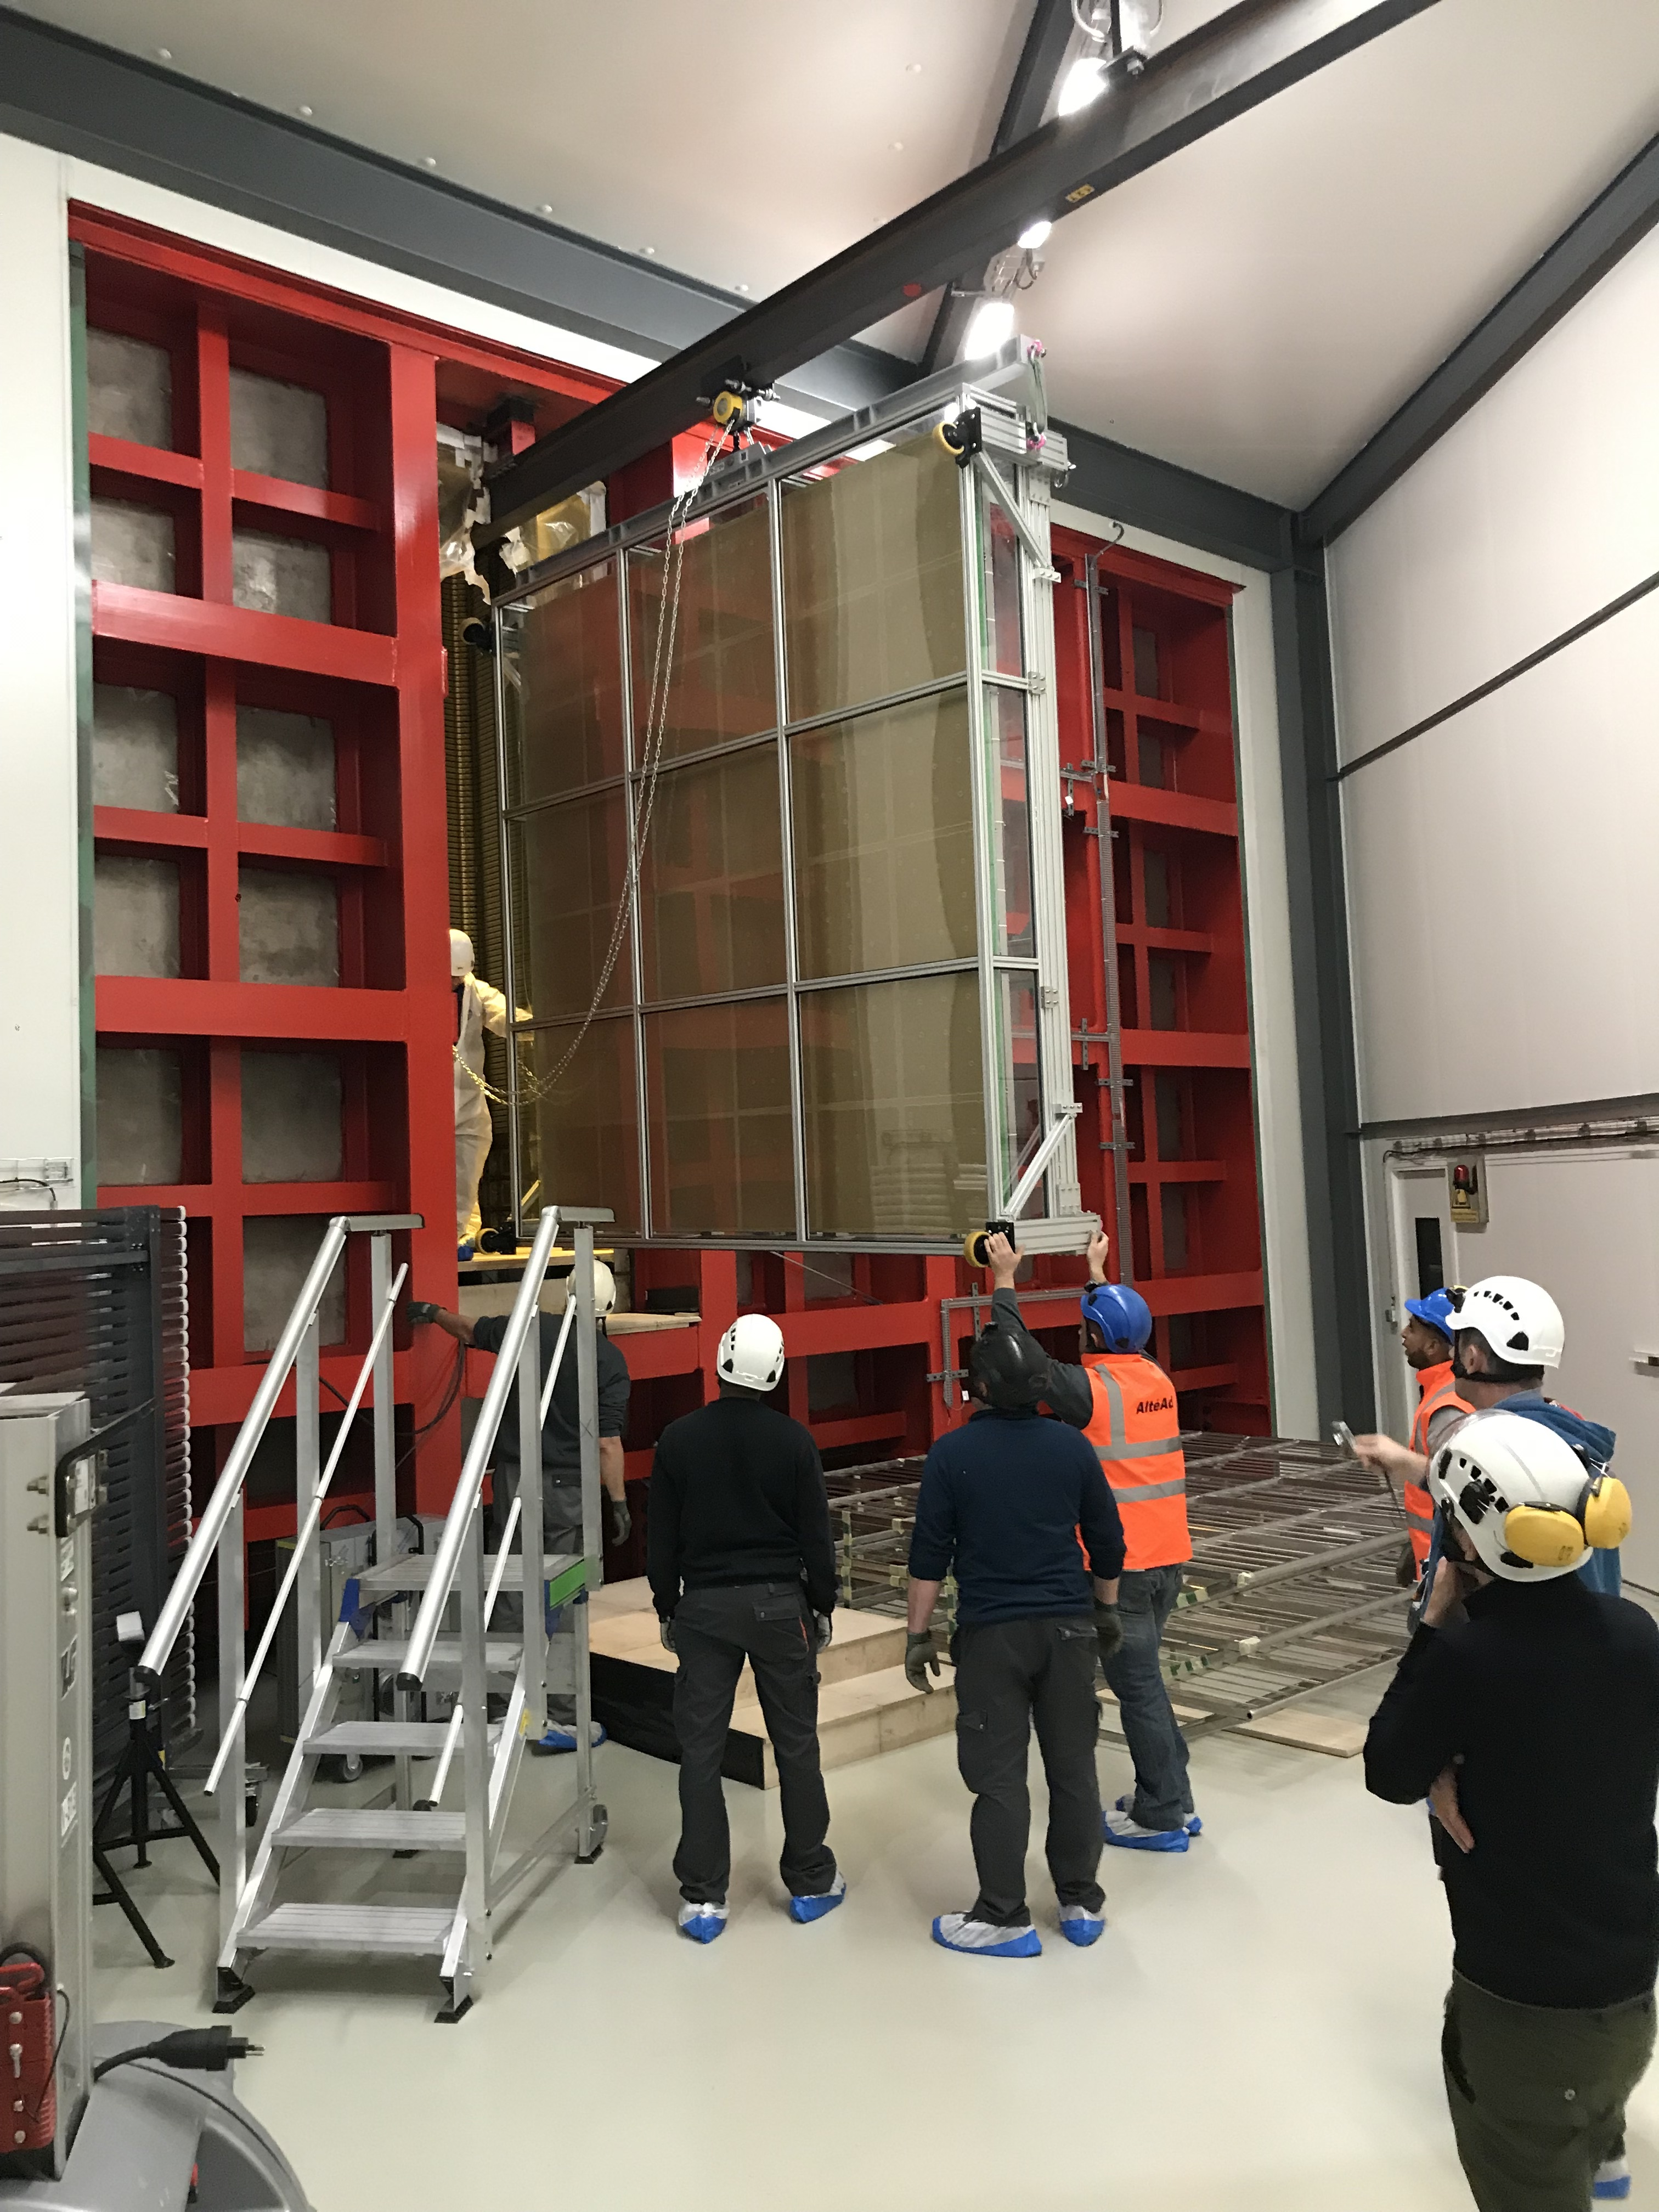
\includegraphics[width=0.45\textwidth]{crpInsertion.jpg}
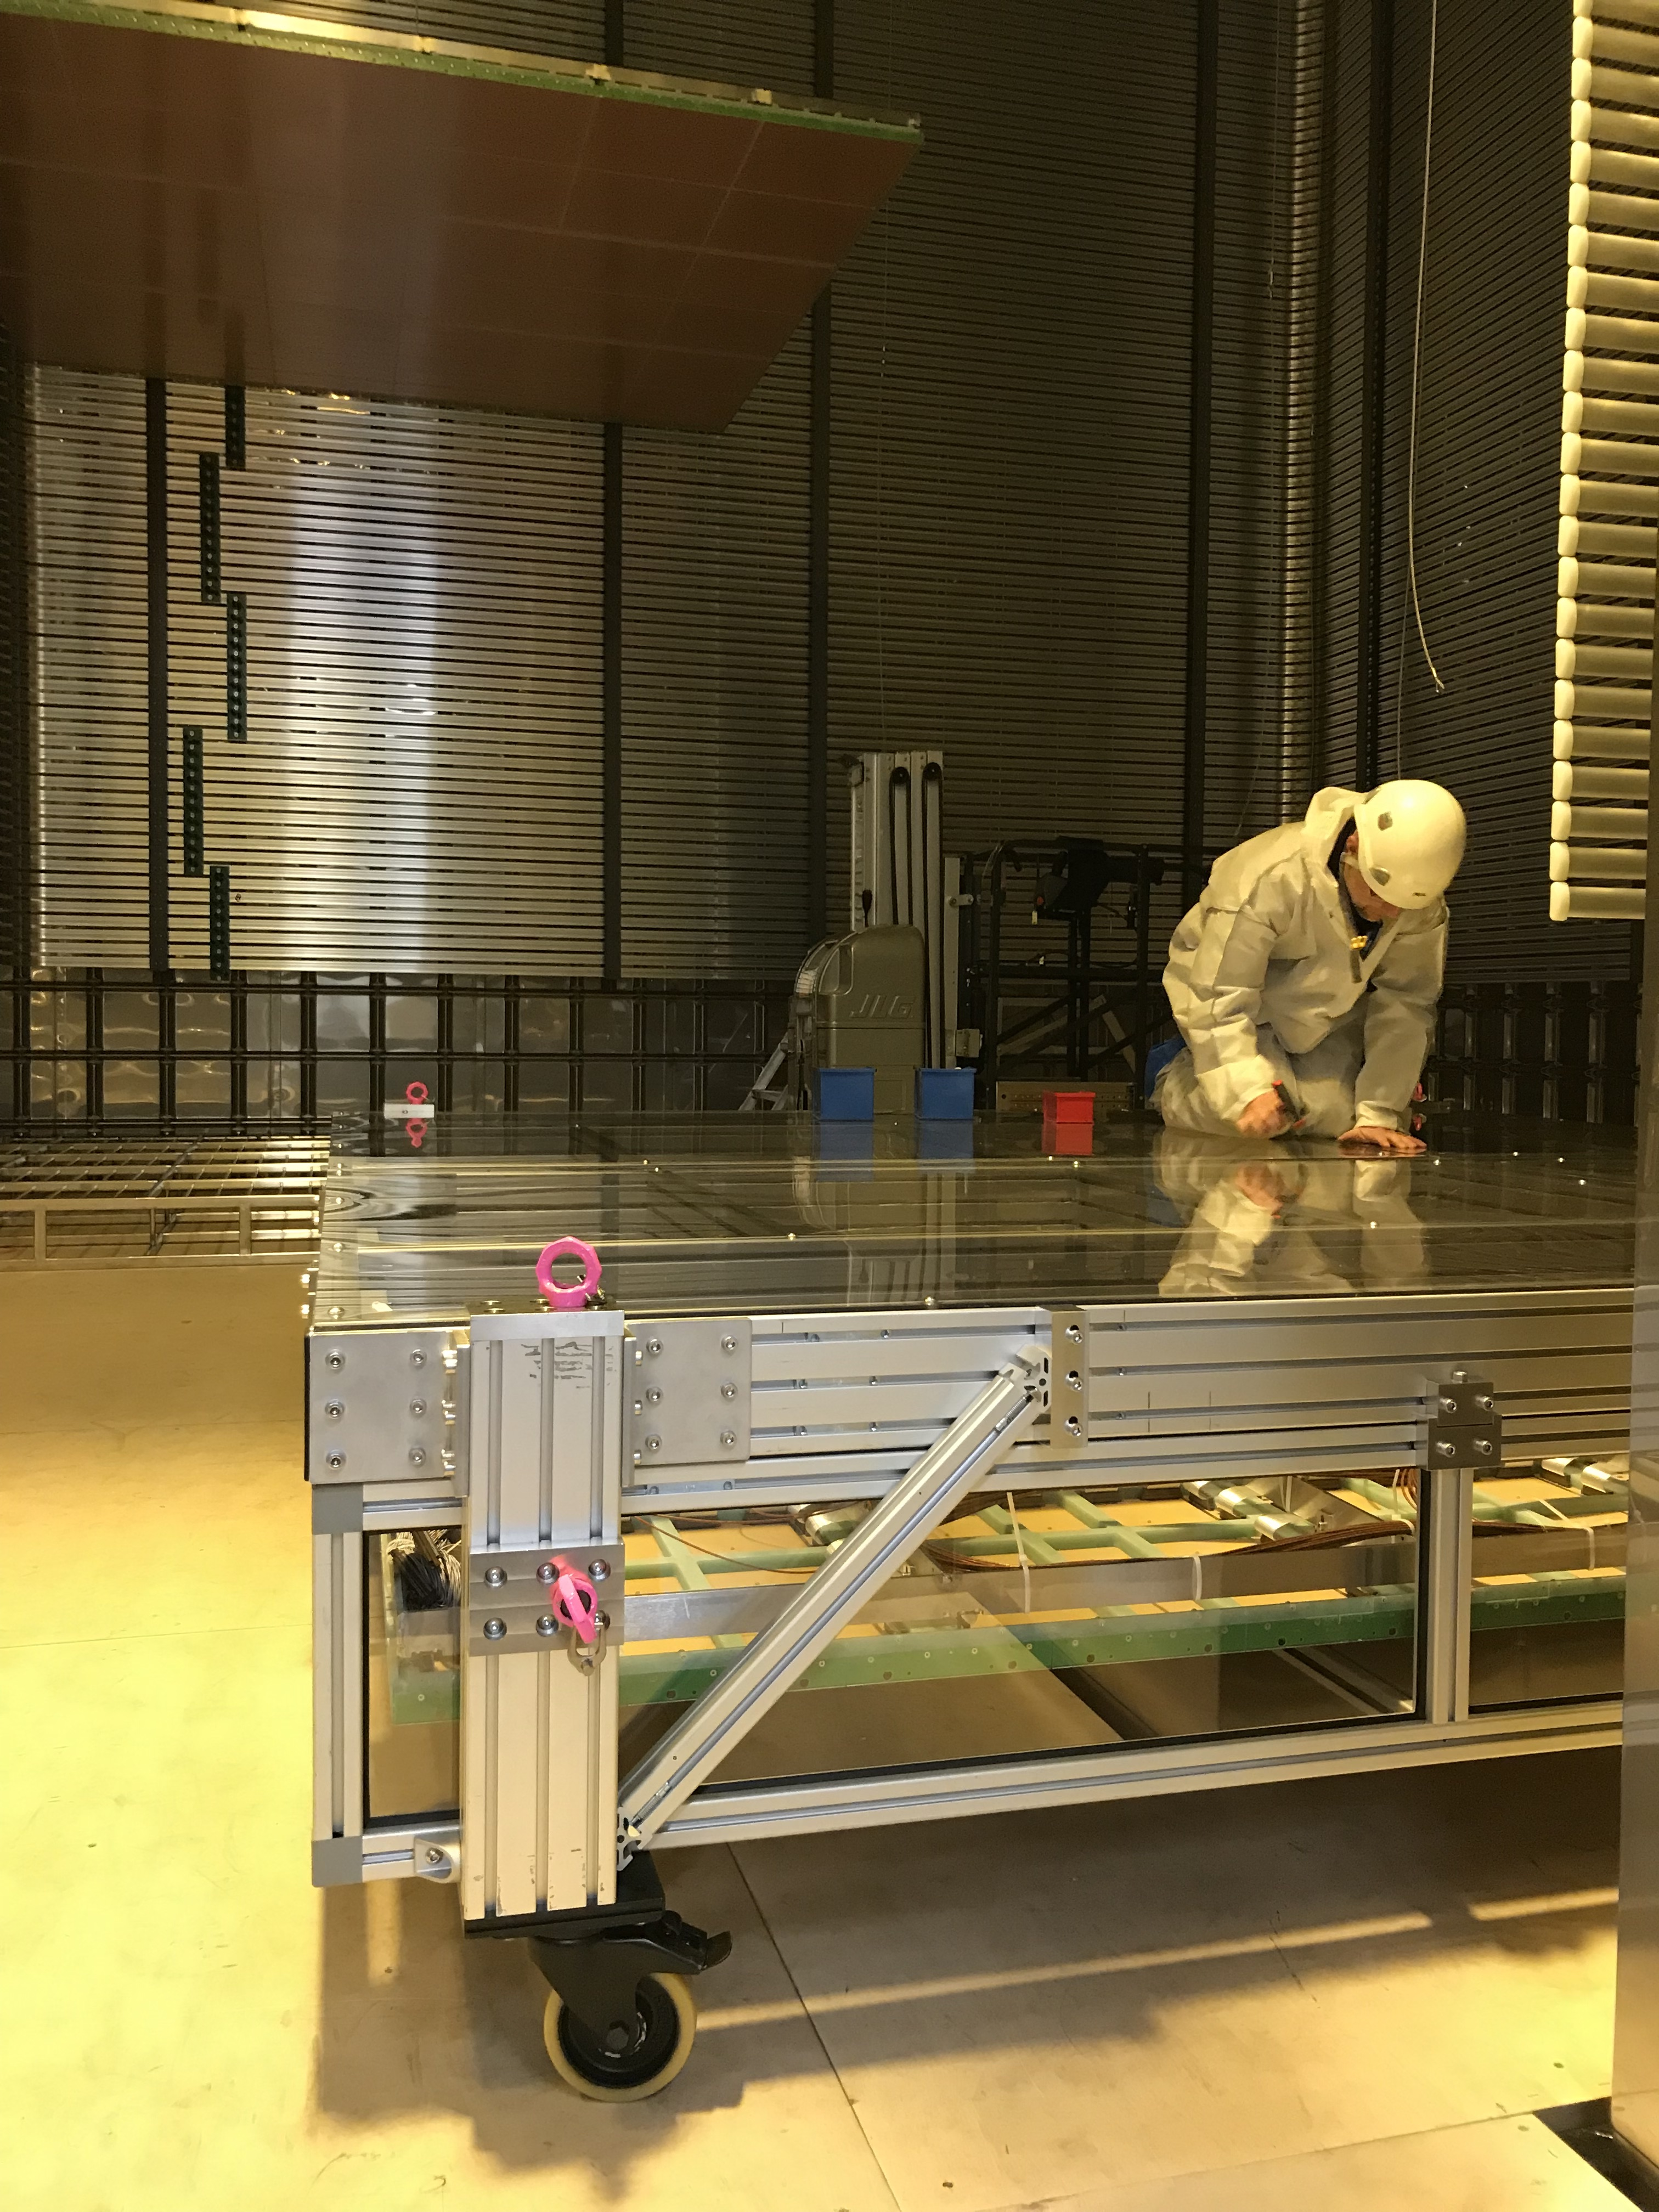
\includegraphics[width=0.45\textwidth]{crpMoving.jpg}
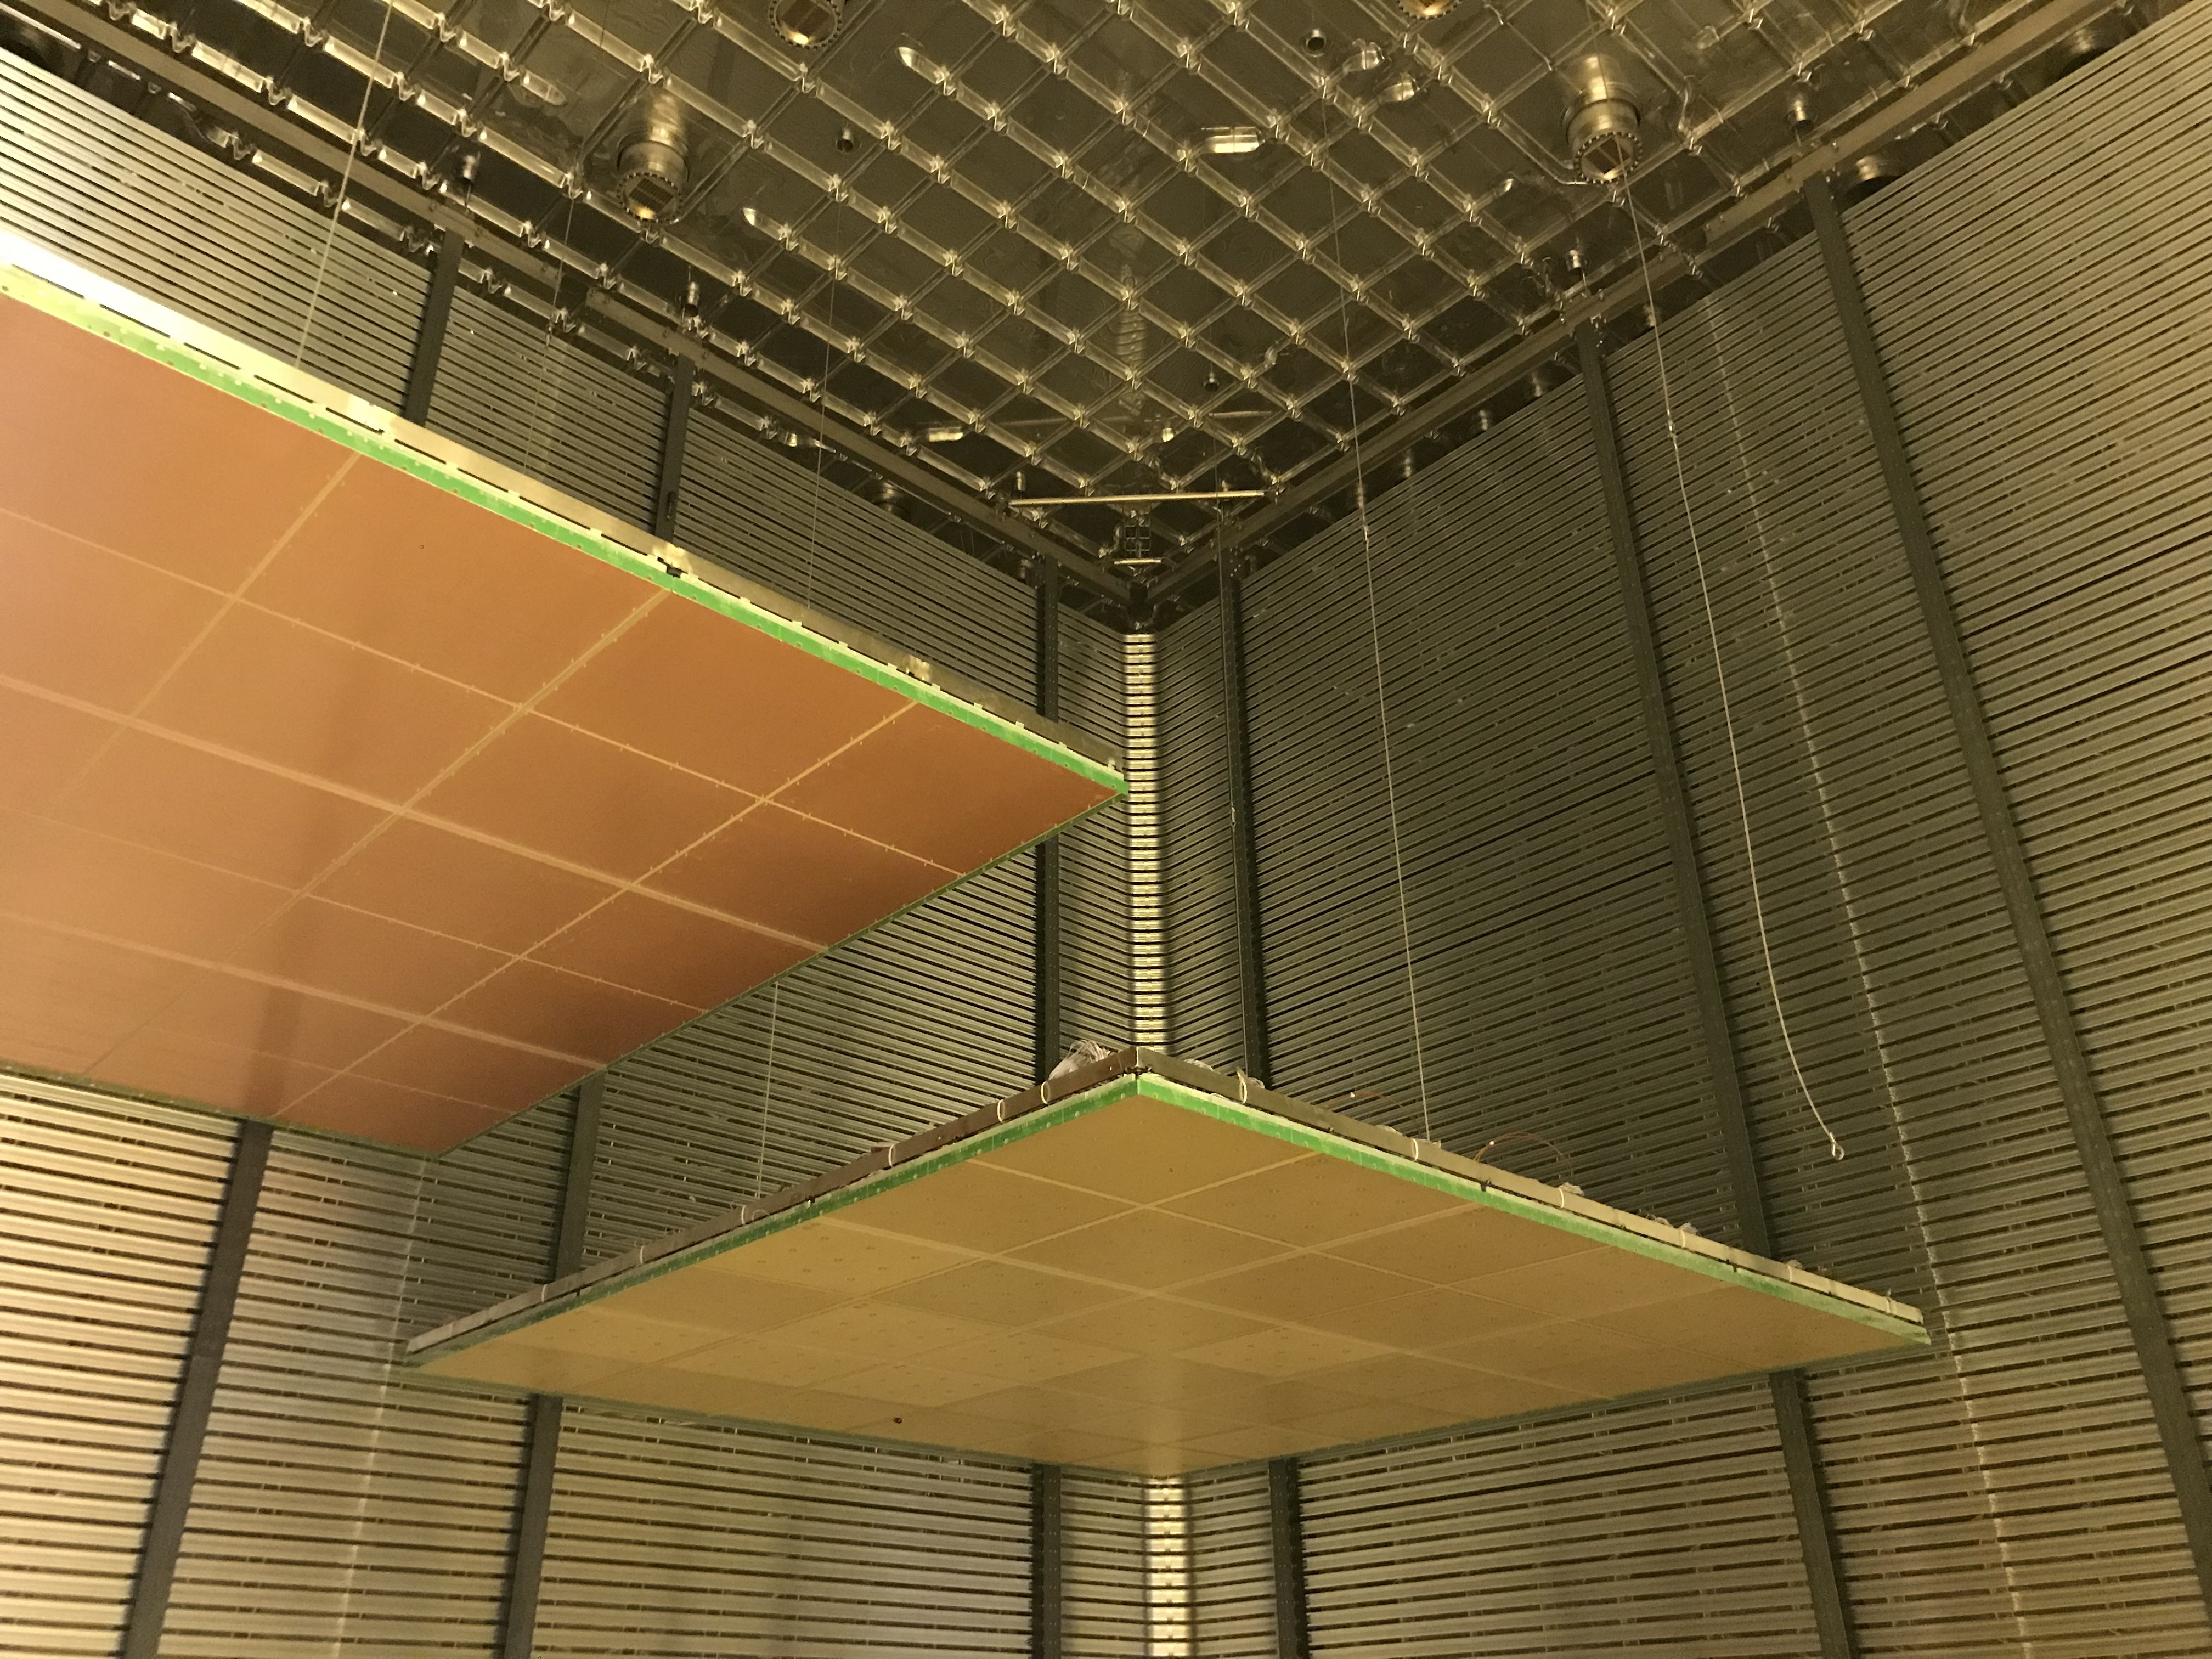
\includegraphics[width=0.9\textwidth]{crpLifting.jpg}
\end{dunefigure}

The installing the 80~\dwords{crp} in the cryostat will take up to ten months.
The signal chimneys underneath the \dword{crp} being installed must be present in order to complete the cabling of the signal cables.
The suspension, instrumentation, and \dword{hv} flanges must also be available.
These components on the roof will be actually installed in parallel with the \dwords{sgft}.
For installation it is foreseen to have enough buffer of \dwords{crp} stored in the vicinity of \dword{surf}.
The installation rate goal is of ten \dwords{crp} installed, cabled, alighted and tested every month.
In order to achieve this goal three teams of two-people in one shift per day are needed.

Provided the means to reach the ceiling for two people, the lifting of one \dwords{crp} in final position is expected to be completed by three people in 0.5 shifts.
The lifting is done from the cryostat roof manually or assisted, depending on the final device available.
The synchronisation of the lifting velocity of the three ropes is fundamental to guarantee the planarity of the \dwords{crp}.
The cabling of the \dwords{crp} is a more complex work.
The position of the \dword{sgft} penetrations and the is \dword{crp} instrumentation penetrations are not always in the optimal position.
The guiding of the cables will be aided by dedicated cable trays and support, but the access, sometimes, will be limited and difficult.
The cabling is done while the \dword{crp} is at the nominal height.
The access between two adjacent CRPs requires staggering the altitude of two neighbouring \dwords{crp} for about 20~cm allowing enough space to do the electrical connections.
This procedure was successfully tested and optimised during the installation of the \dword{pddp}.
The cabling must be followed by a scrupulous and prolonged tests of the connections.
This means that even if the final electronics adn power supplies are not finally installed and functional, the \dword{crp} and the cold electronics consortia engages the responsibility of assuring the quality of the connections. 
Optimising the cable bundles one can assume that the cabling of the signal cables for one \dword{crp} is completed by two people in 0.5 shift.
The cabling of the \dword{crp} instrumentation is completed from the inside of the cryostat by two people in 1 shift.
If the \dword{lem} \dword{hv} feedthrough is the same as the one of \dword{pddp}, the finalisation of the connection will take 2 shifts for a person.
The testing of the \dword{lem} \dword{hv} characteristics when installed is a complex issue because the drawn current and the discharge probability depend on the air quality, and above all on the humidity level that at present there is no plan to control.
The \dword{hv} behaviour of the installed \dwords{lem} must be followed for a significantly amount of time soon after the installation (days), and repeated regularly.
The first test must be done before the installation of the cathode underneath the \dword{crp} is done: In case of issues the \dword{crp} is reachable without major intervention and disassemble of other detector components.
Therefore, the \dword{hv} tests on the \dwords{lem} are carried on while the \dwords{crp} are still being installed.
A procedure to guarantee the safety of the personnel must still be detailed.
When $4 \times 4$ island of \dwords{crp} are completely installed and before the cathode is in place, a global survey of the 16~\dwords{crp} must be done in order to level them at the nominal position.



Each \dword{crp} will be tested underground in the cold box to characterise its electrical and mechanical behaviour in cryogenic conditions.
Figure~\ref{fig:crpTestingSchedule} shows a plausible schedule for tests in the four cold boxes.
The staggering of the cold box operation is ideal, and very difficult to maintain.
For this reason, the operation of each cold box is meant to be independent.
The time allocated for the opening and the closing procedures is extented by a factor two to compensate possible delays due to activities on two cold boxes involving the clean room crane at the same time.
In the planing, the installation of the \dword{crp} under the roof of the cold box and the closure of the cold box is allocated in one shift.
Crane drivers (two) will be the main actors in this activity.
From the \dword{pddp} experience, the time it takes to connect the \dword{crp} below the cold box roof, open the transport box, and close the cold box is four hours for two riggers, one \dword{crp} expert, and one technician.
Always based on \dword{pddp} experience, the time allocated for the cool-down and filling of the cold box is two days.
One cryogenic expert is expected to be on shift and supervise the activities for the four cold boxes (the ability to intervene 24~h/day on cryogenic parameters - most importantly to act on the liquid argon level - is unavoidably).
\dword{crp} and \dword{lem} experts are expected to perform the characterisation in three days.
Two experts per shift will be able to follow the operation of the four cold boxes.
As in the case of \dword{pddp} cold box tests, during the nights the experts should be able to intervene remotely in case of issues.
The time allocated to empty the cold box and warm it up is two days.
Similarly to the cold box closure, one shift is allocated to open the roof and put the \dword{crp} back in his transport box ready for installation.
One contingency day is considered for each cold box test cycle.
On average 2.5~days will be needed to install and connect the \dwords{crp} inside the cryostat by a group of at least three technicians and one \dword{crp} expert.
An initial period of ramp up, where fewer than four cold boxes are operational, is expected.
A plausible time line of the number of \dword{crp} tested in each cold box is shown at the bottom of figure~\ref{fig:crpTestingSchedule}.
It is believed that on a schedule of one shift per day seven days per week, the \dwords{crp} will be installed in about 8 months.
The contingency in the test and installation considered in this schedule allow for repairs of minor issues found during the tests.
In the global schedule, the installation of the \dwords{crp} takes 9 months.
This is done to take into account the improbable case where a major issue in up to four \dwords{crp} is found, and these \dwords{crp} must be transported to the surface and shipped back to the factories.
It is also believed that the time needed to test and install the \dwords{crp} will reduced the more \dwords{crp} are tested.

\begin{dunefigure}[Schedule of the \dshort{crp} tests in the \coldbox{}es]{fig:crpTestingSchedule}
{Schedule of the \dword{crp} tests in the four cold boxes and the number of \dword{crp} tested in each cold box.}
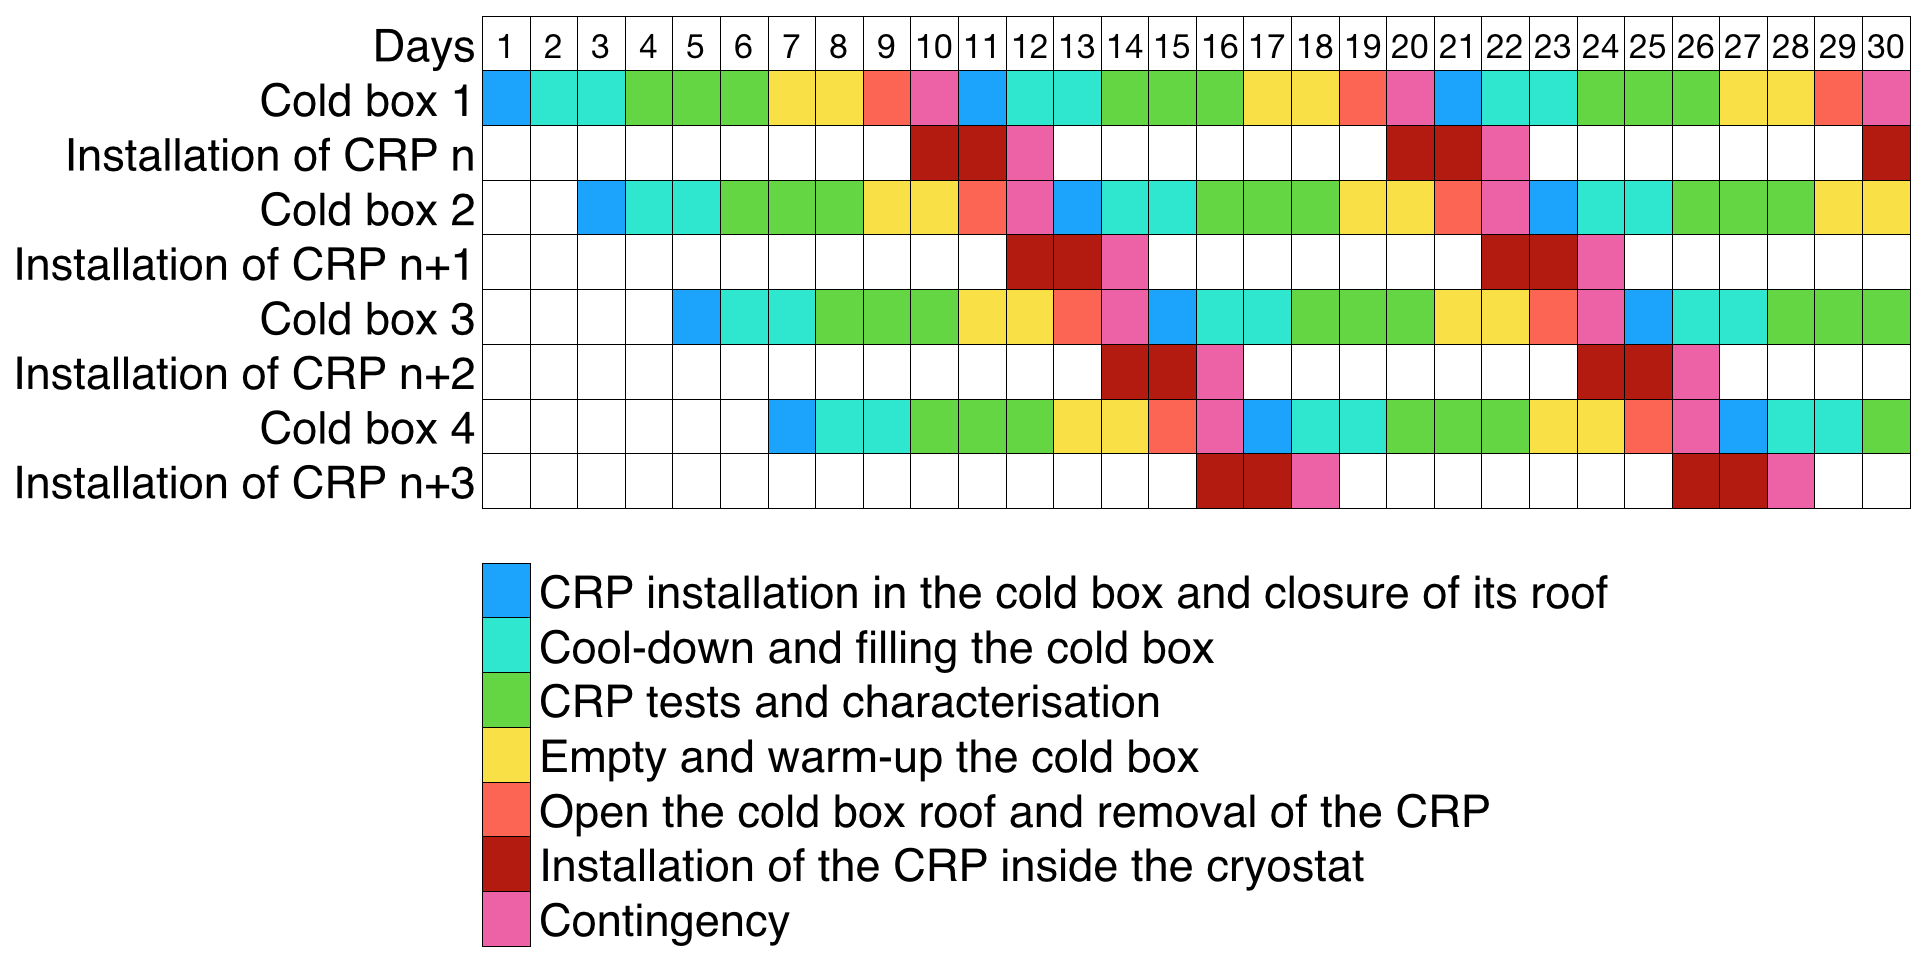
\includegraphics[width=0.8\textwidth]{crpTestingSchedule.png}
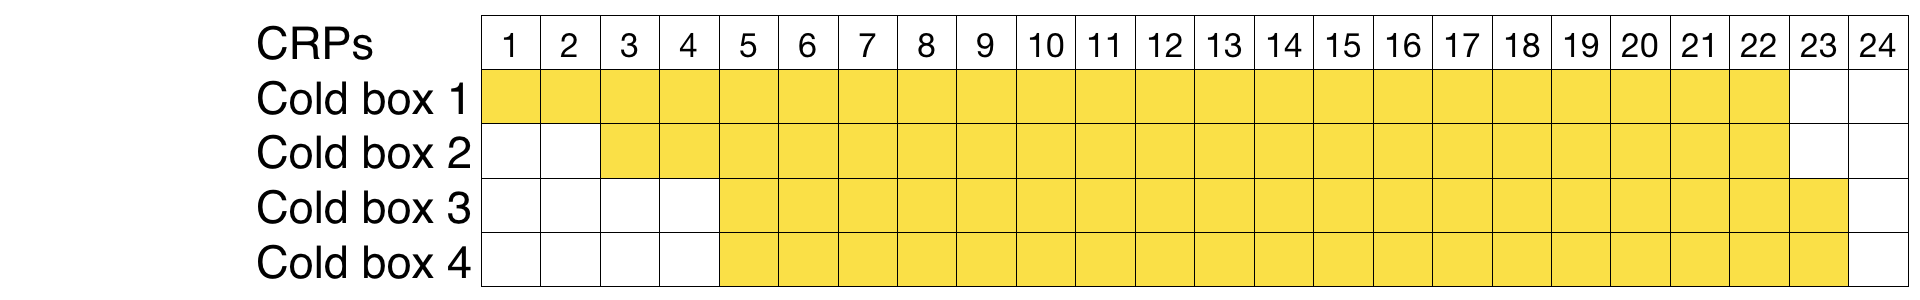
\includegraphics[width=0.8\textwidth]{crpTestDeliveries.png}
\end{dunefigure}


\subsection{High voltage system installation}
Most of the \dword{hv} components installed inside the cryostat will actually be assembled underground.
The reason for this choice is to optimise the transport and storage, considering the fact that the assembly of the \dword{fc} and cathode are not a very resources consuming activities that can be done in parallel with the installation of the \dwords{crp} and \dword{hv} system.

The \dword{fc} \dword{frp} I-beams and the stainless steel cross bars are shipped in standard wooden crates in a very compact fashion.
The components for each \dword{fc} sub-module are packed into one compact flat pack $0.1 \times 0.1 \times 2$~m$^2$ and sealed in several layers of shrink wrap and a thick, soft cushion of plastic layers for edge protection.
Because each sub-module package is so compact, each wooden crate of $1.5 \times 1.3 \times 2.5$~m$^3$ can contain up to 110~sub-module flat packs stacked.
Excluding spares, the total number of sub-module flat packs needed for the entire \dword{fc} is 216, there fore only two crates are needed for a total weight of less than 5~ton, that will be stored underground.

The extruded aluminum profiles for \dword{fc} are shipped separately in standard wooden crates.
In all, 199~4~m-long profiles are needed for each 12~m-long \dword{fc} module, for a total of 7164~profiles to transport underground, excluding spares.
The same number of resistive sheaths are shipped separately.
The 12~m (L) 30~cm (H) 2.5~cm (W) trusses for the cathode modules are shipped to \dword{surf} in transport containers, while the 12~m (L) 2.5~cm (D) resistive rods are shipped in standard wooden boxes.
The installation procedure takes into account the lack of storage space at the 4850~level.
The cathode modules are transported underground in an assigned order, corresponding to their installation sequence starting from the end of the cryostat opposite the \dword{tco}.

The power supply, the \dword{hv} feedthroughs, and \dword{hv} extender are sent to \dword{surf} in standard shipping crates and brought underground when installation requires.

The \dword{fc} is divided in twelve super-module of $12\times12$~m$^2$, five along each long side wall and one along each end-wall.
Each super-module is built out of 18~sub-modules installed in $3 \times 6$ matrix.
The three topmost sub-modules interface with the 12~m-long stainless steel beam from where the entire super-module is hanging.
The three sub-module at the bottom connects with the cathode.

The \dword{fc} sub-modules are assembled inside the \dword{dpmod} cryostat, in a dedicated area of about $5 \times 4$~m$^2$ towards the \dword{tco}.
The completed sub-modules are stored inside the cryostat until they are assembled in the super-module.
The area is large enough for assembly, storage of the sub-modules prior final installation and still allowing comfortably the passage of material and people inside the cryostat.
An assembly table with a precision alignment bar is used for the rapid profile positioning.
The sub-module package is cleaned in the clean room before being brought inside the cryostat by means of the same crane used to insert the \dwords{crp}.
The package is opened on the alignment table and the mechanical frame is assembled from two \dword{frp} I-beams and two stainless steel tubes.
Once the frame is assembled, the aluminum profiles are mounted on the flange of the \dword{frp} I-beams and secured using two slip nuts inserted on either end and are secured with two button-head, hex-drive metal screws, with one side secured tightly and the other loosely, but solidly, in order to avoid stresses due to thermal contraction.
Care must be taken to avoid scratching the profiles during the mounting process.
The resistive sheaths for sub-module interconnections and the square nuts to hold \dword{hvdb} are pre-inserted to each profile at the assembly stage.
All the screws are tightened with the right and reproducible torque using a power screwdriver with a preset torque.
A base with wheels constructed out of unistrut bars is mounted to the bottom of the sub-module, to allow easy handle and transport inside the cryostat to the designated installation section.

When three top sub-modules, three bottom sub-modules, and twelve middle sub-modules are assembled, they will be installed as a super-module starting at the far end of the cryostat.
The installation sequence is thought to avoid the need of working an height higher than 3~m.
The installation for a super-module follow the following steps:
\begin{enumerate}
\item Hang the 12~m-long stainless steel I-beam from two stainless steel cables through the feedthroughs and lift it to approximately 2.5~m above the temporary floor and secure it at this position.
The lift is done from the roof of the cryostat with manual winches in a similar way as done for the \dwords{crp}.
The team inside the cryostat will guide the lifting operation of the team on the roof.
Effective communication between the inside and outside of the cryostat is crucial for this operation.
Walkie-talkies were effectively used for this purpose during \dword{pddp} installation.
Before the stainless steel I-beam is transported inside the cryostat they are cleaned in the clean room.
The time spent inside the clean room is less than 0.5 shift.
The ongoing activities in the celan room should therefore not be perturbated by the cleaning and insertion of the I-beam inside the cryostat, provided that this operation should not be done when the cold boxes are opened or closed.
The stainless steel I-beam is transported inside the cryostat as for all the other items, and it is transported in the installation point by means of carts rolling on the false floor.
\item Place three top sub-modules under the stainless steel I-beam and connect each to the I-beam using two sets of stainless steel L-brackets, stainless steel inserts, stainless steel screws, stainless steel lock washers, and stainless steel nuts.
\item Slide the two resistive sheaths (pre-inserted into the middle sub-module) over and tighten them onto the two neighbouring profiles to make the resistive connections between profiles in the same row.
\item Mount \dword{hvdb} to the center sub-module in the row, using aluminum button-head screws and a square nut pre-inserted in the profile reinforcement rail.
This operation completes one row of the sub-modules for a super-module.
\item Mount the reflector/\dword{wls} panels for the photon detection system to cover completely the first row of sub-modules towards the active volume.
\item lift the completed top row by approximately additional 2.5~m and secure the super-module in this position.
Place three middle sub-modules under the top row, and connect each to the corresponding top sub-module above using 1~cm thick connection plates and stainless steel screws and nuts.
Repeat the relevant steps described above to install all the six raws of sub-modules.
The first three are equipped with the reflectors.
\end{enumerate}

Work at the level of the cryostat ceiling is required in order to connect the super-module to the final anchoring system and release the temporary lifting ropes.
This operation can be done from the inside of the active volume using the man lift as long as the \dwords{crp} in that region are not installed.
Additional work at height is needed to connect the safety ground connection of the topmost field shaping ring with the cryostat wall/ceiling and to connect the topmost field shaping ring power to the dedicated feedthrough port.
Again this activity should be done as last steps of the installation of the super-module with a man lift.

Figure~\ref{fig:fieldCageInstallation} shows a moment in the installation of the \dword{fc} in the \dword{pddp}.
For what concerns the installation sequence, the most relevant difference between the \dword{pddp} (other than the total height of the modules) is the fact that the super-module consisted of one single raw of sub-modules.
In figure~\ref{fig:fieldCageInstallation} the super-modules are still hanging from the temporary lifting stainless steel ropes.
The wheel base carts below the sub-modules are visible.
\begin{dunefigure}[\dshort{pddp} field cage installation]{fig:fieldCageInstallation}
{Installation of the \dword{pddp} field cage.}
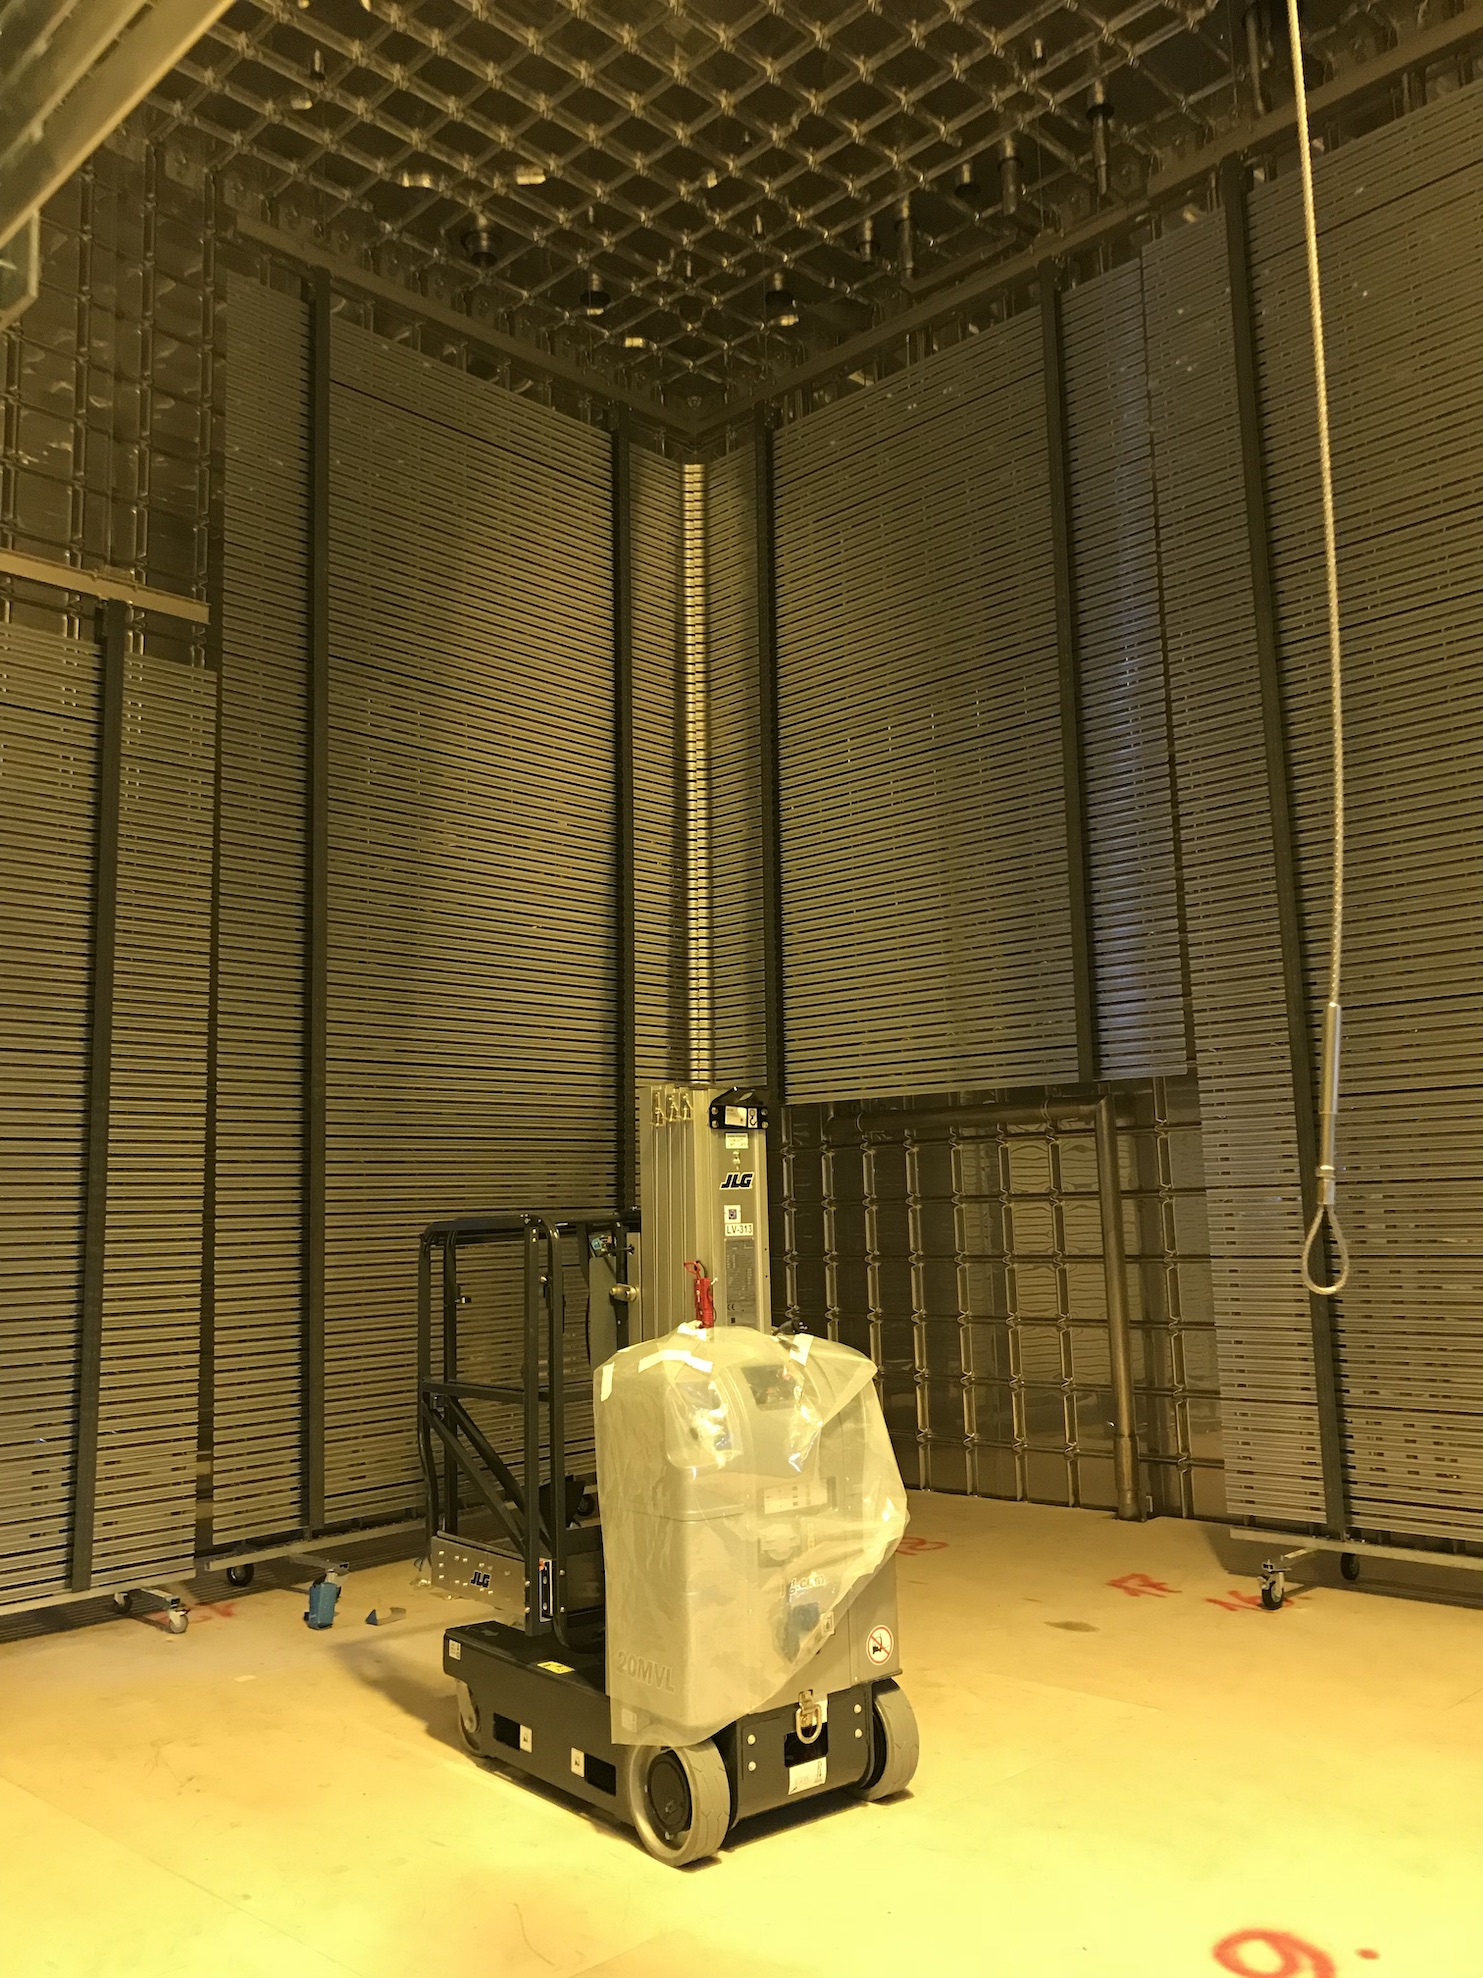
\includegraphics[width=0.9\textwidth]{fieldCageInstallation.jpg}
\end{dunefigure}

The cathode consists of 15~sections of $4 \times 12$~m$^2$ to cover the length of 60~m of the \dword{dpmod} \dword{tpc}.
They are installed hanging from the bottom of the \dword{fc} connecting the two long walls.
Each section consists of two 12~m-long trusses made from thin-walled stainless steel tubes with approximately 50~mm outer diameters.
They can either be prefabricated and transported underground like the large cryostat I-beams or assembled in the underground area from sectional parts.
They must be un-boxed and cleand inside the clean room before entering into the cryostat.
The trusses are 2~m apart and are connected at both ends to stainless steel tubes that run under the \dword{fc} and form the outer tube ring of 144~m surrounding the cathode plane.
The actual cathode plane consists of 10~mm diameter resistive rods installed at a pitch of 10~cm through holes in the straight upper tubes of the trusses.
The \dword{fc} end-wall must be pushed about 50~cm towards the inside of the active volume to meet the \dword{fc} side walls and cathode to form a trapezoidal section of the active volume.
This is required to move away the cathode from the cryostat walls and meet the maximum field specification inside the liquid argon.

The ground grid that protect \dwords{pd} from the high electric field consists of 80~self sustained modules made out of stainless steel.
They are installed with four legs directly on the corrugated floor with teflon sheets to protect it from scratces.
The legs can be extended to allow confortably the installation of the \dwords{pd}.
The position of the legs matches the flat part of the corrugation adn avoid the \dwords{pd} and the internal cryogenic lines.
The ground grids are light enough that can be transported and handled manually by two people and installed by four people.
For more details see the \dword{hv} chapter of this \dword{tdr}.

The entire \dword{hv} system, including \dword{fc}, cathode, ground grid, and the reflector/\dword{wls} panels are installed in the following sequence:
\begin{enumerate}
\item Construct the end-wall super-module (equipped with the 90~degree bent corner profiles) at the end of the cryostat opposite to the TCO.
\item Mount the U-shaped stainless steel cathode end-wall perimeter tube to the bottom of the end-wall super-module.
\item Install the two super-modules along the side wall immediately next to the end-wall module.
\item Make the electrical connections to the end-wall super-module.
\item Pull in the bottom of the end-wall super-module about 50~cm from its free hanging position in order to align its profiles to the ones of the wall \dword{fc} super-modules. Secure the end-wall super-module to the temporary false floor.
\item Electrically connect the end-wall super-module and side wall super-modules using the pre-inserted resistive sheath.
\item Assemble the cathode module in place at the bottom of the two side \dword{fc} modules immediately next to the end-wall super-module.
Special lifting equipment is foreseen to manipulate the cathode and lift it in position to allow simple connection to the~\dword{fc}.
\item Connect the stainless steel perimeter cathode tube already mounted on the end-wall super-module to the corresponding cathode tubes on the side wall super-modules, and anchor it to the false floor to ensure the mechanical stability of the end-wall super-module until the entire \dword{fc} is constructed.
\item Once the cathode section is securely hanging from the \dword{fc}, remove the temporary floor under the cathode, and clean the membrane floor.
\item Place the ground grids under the cathode plane with their legs extended and start the installation of the \dwords{pmt}.
\item Once the \dwords{pd} installation is completed and cabling is complete below one ground grid, remove the leg extensions of the ground grid and lower it to the nominal height.
\end{enumerate}
Figure~\ref{fig:groundGridInstallation} shows the installation in \dword{pddp} of the ground grid above the \dwords{pmt} already in final position.
In this case, four $3 \times 3$~m$^2$ sections of the ground grid where installed.
The sections had to be connected to each other, they where not independent.
From the installation point of view ground grid in the \dword{dpmod} will be simpler to install compared to the \dword{pddp} also because the ground grid frame between the cryostat walls and the main ground grid, present in \dword{pddp}, will not be installed in \dword{dpmod}.

\begin{dunefigure}[Installation of the ground grid above the \dshorts{pmt} in the \dshort{pddp}]{fig:groundGridInstallation}
{Installation of the ground grid above the \dwords{pmt} in the \dword{pddp}.}
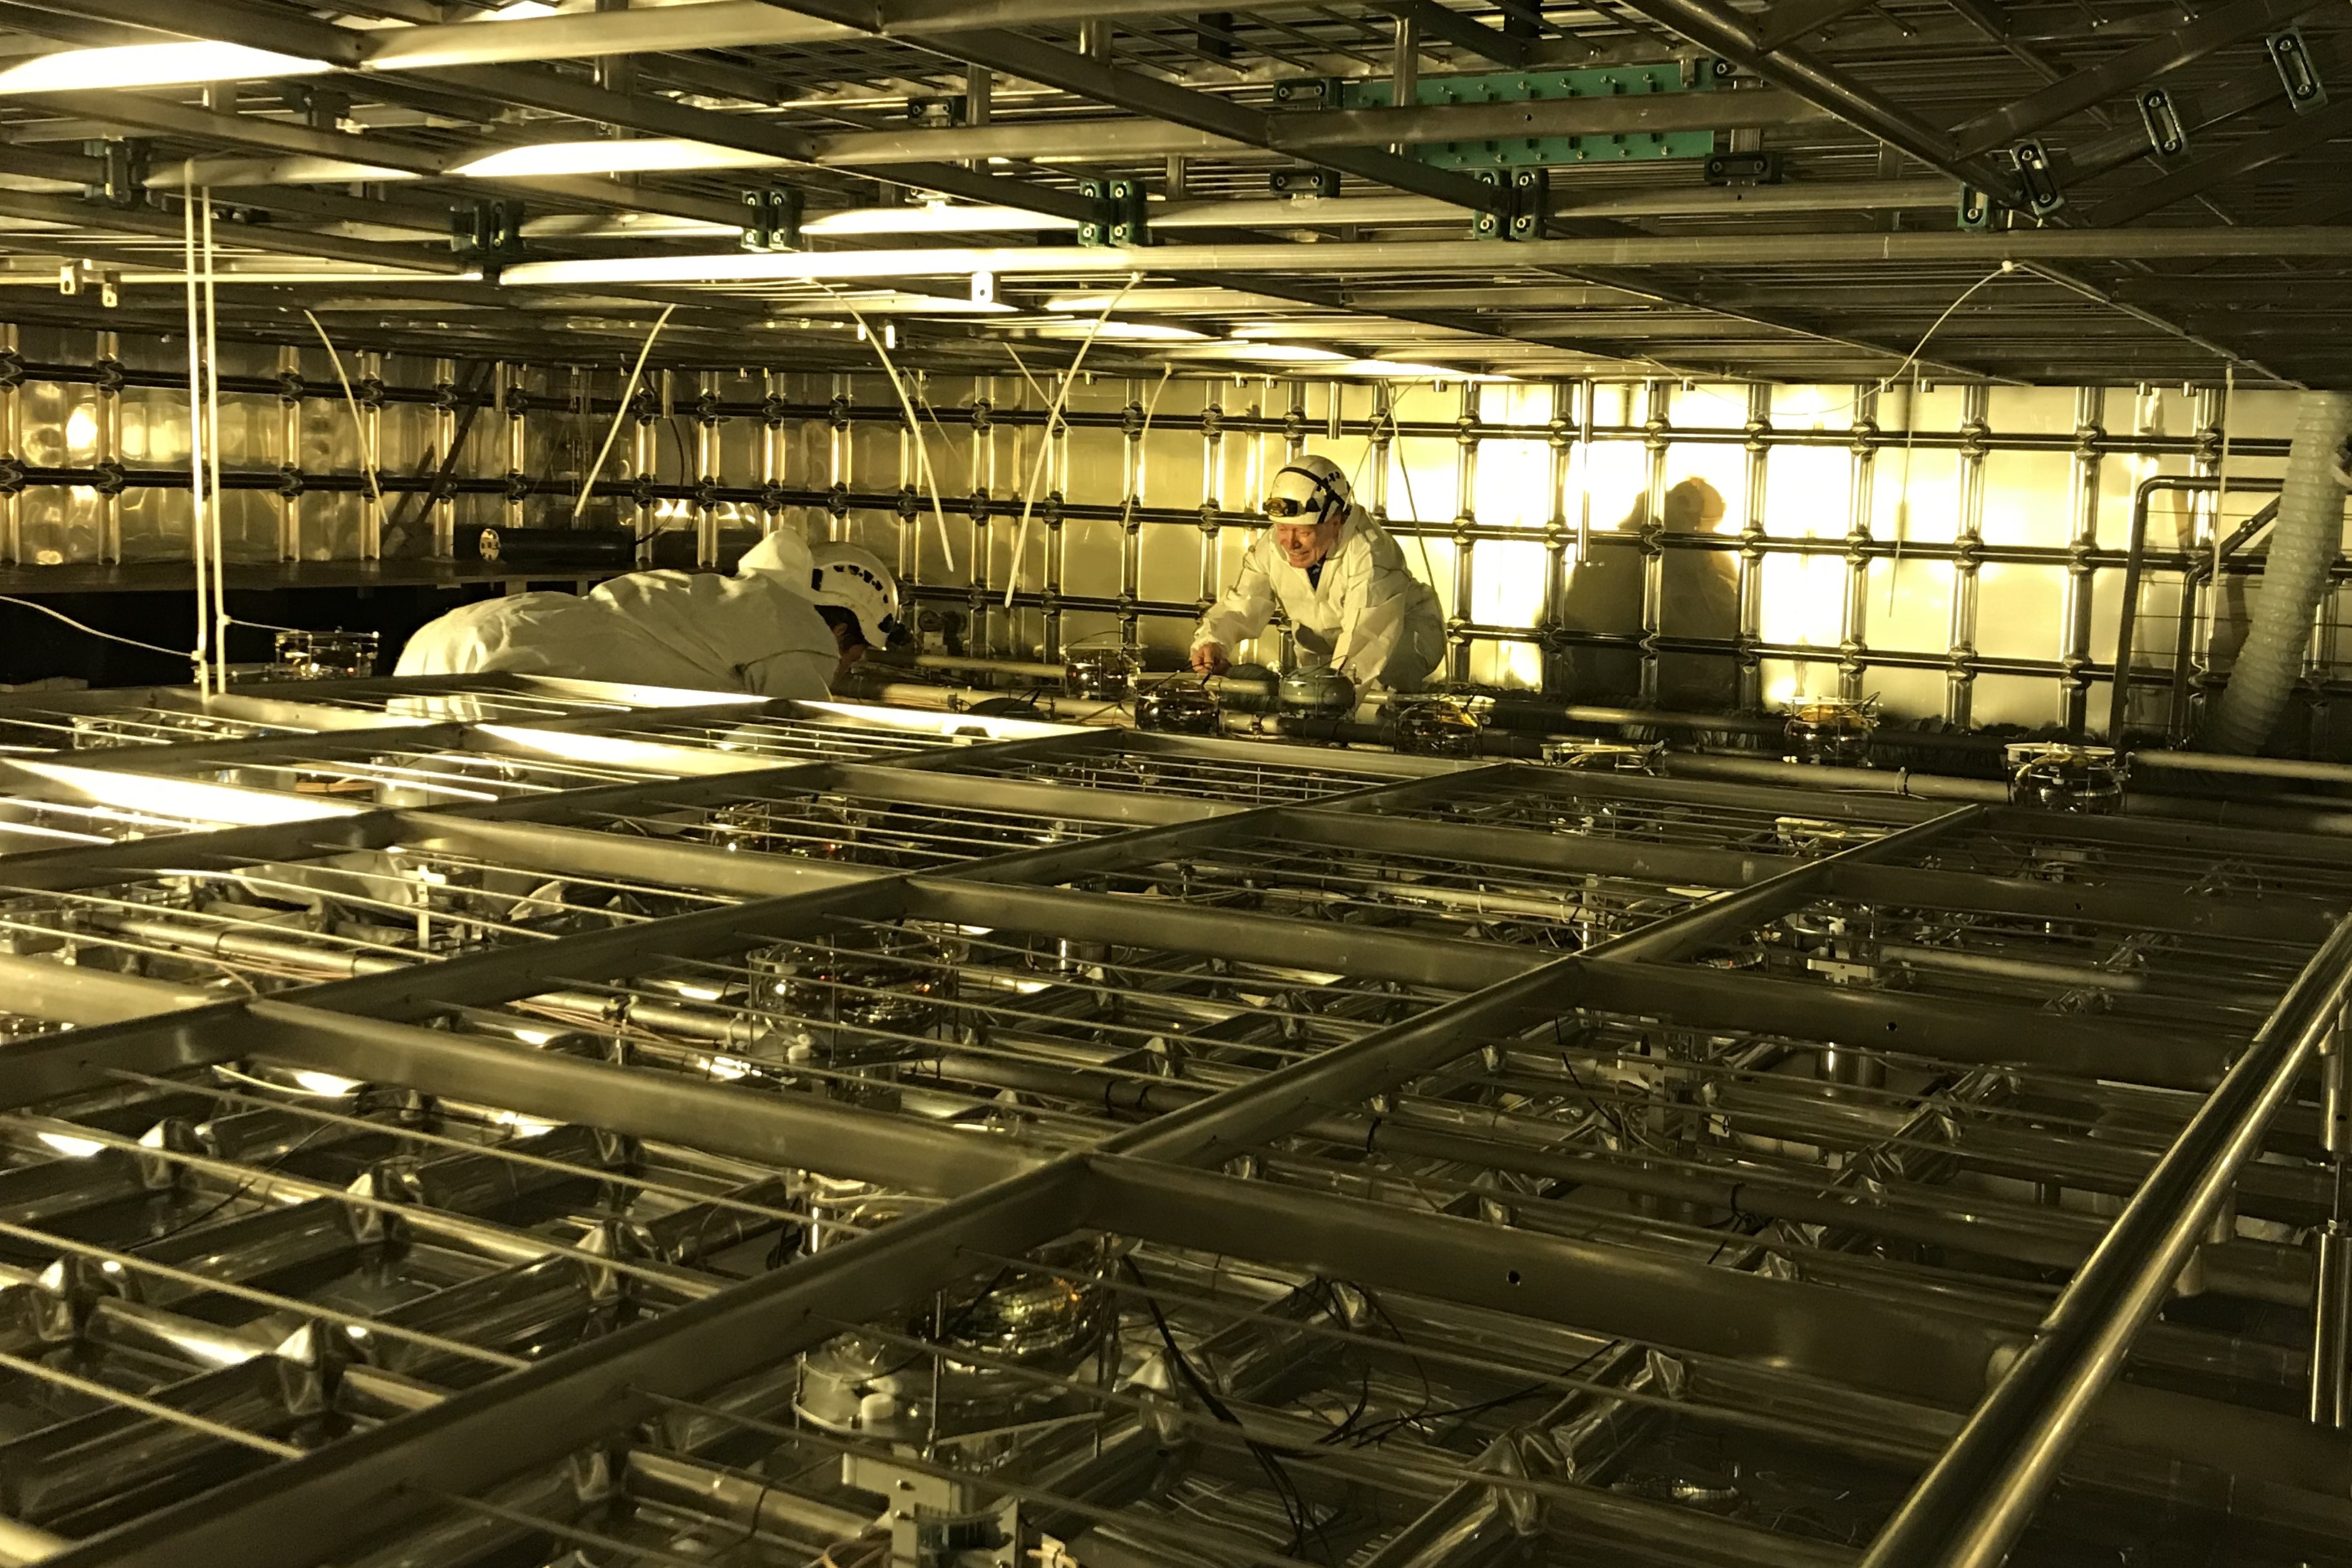
\includegraphics[width=0.9\textwidth]{groundGridInstallation.jpg}
\end{dunefigure}

What was described above is the procedure that is valid until the installation of the \dword{tco} end-wall.
To assemble the end-wall super-module as the others, all the \dwords{crp} must be installed first and all the sub-modules for the last super-module must be available inside the cryostat stored on the false floor around the active volume.
The man lifts needed for the installation of the \dwords{crp} are too tall to pass below a fully installed end-wall to being finally extracted from the cryostat.
In \dword{pddp} the bottom-most sub-module of the super-module in front of the \dword{tco} was not installed.
This was possible because the super-module consisted of a single raw of sub-modules.
The activities at the ceiling level for what concerns the last end-wall will be carried out using a scaffold.
Once the end-wall is in place, the \dword{hv} extender that that was inserted into the cryostat prior the installation of the end-wall,
is installed.
As per the actual design, the extender is a 12~m-long rigid cylinder with an inner conductor and outer field shaping rings.
Its role is to create an electrical connection between the tip of the feedthrough, that is installed as last thing, and the cathode without too much distorting the drift field in its vicinity and guaranteeing a maximum electric field inside the liquid argon below 30~kV/cm.
For the installation, the extender (unpackedn and cleaned) is laid horizontally on a portion of false floor left free of the scaffold.
It is lifted vertically with a pulley and a rope passing through the \dword{hv} feedthrough.
It is finally secured to the anchoring mechanism welded on the penetration pipe.
The extender pass through a special \dword{crp} that leaves a corner without anode, \dwords{lem}, grid or any other mechanical obstacles.
Figure~\ref{fig:extenderInstallation} shows this operation done in the \dword{pddp} with the 6~m-long extender, which in that case was installed outside the active volume (no special \dword{crp} was needed).
Once all the electrical connections of the \dword{hv} system are established, a global continuity test will be conducted applying voltage at the cathode through the \dword{hv} feedthrough and measuring the current drawn.
Monitor the voltage and current will be an exercise repeated regularly before the beginning of the gas argon purge, and it will constantly done during purge, cool-down and filling. 
\begin{dunefigure}[Installation of the \dshort{hv} extender in the \dshort{pddp}]{fig:extenderInstallation}
{Lifting of the \dword{hv} extender from horizontal to vertical position in the \dword{pddp}.}
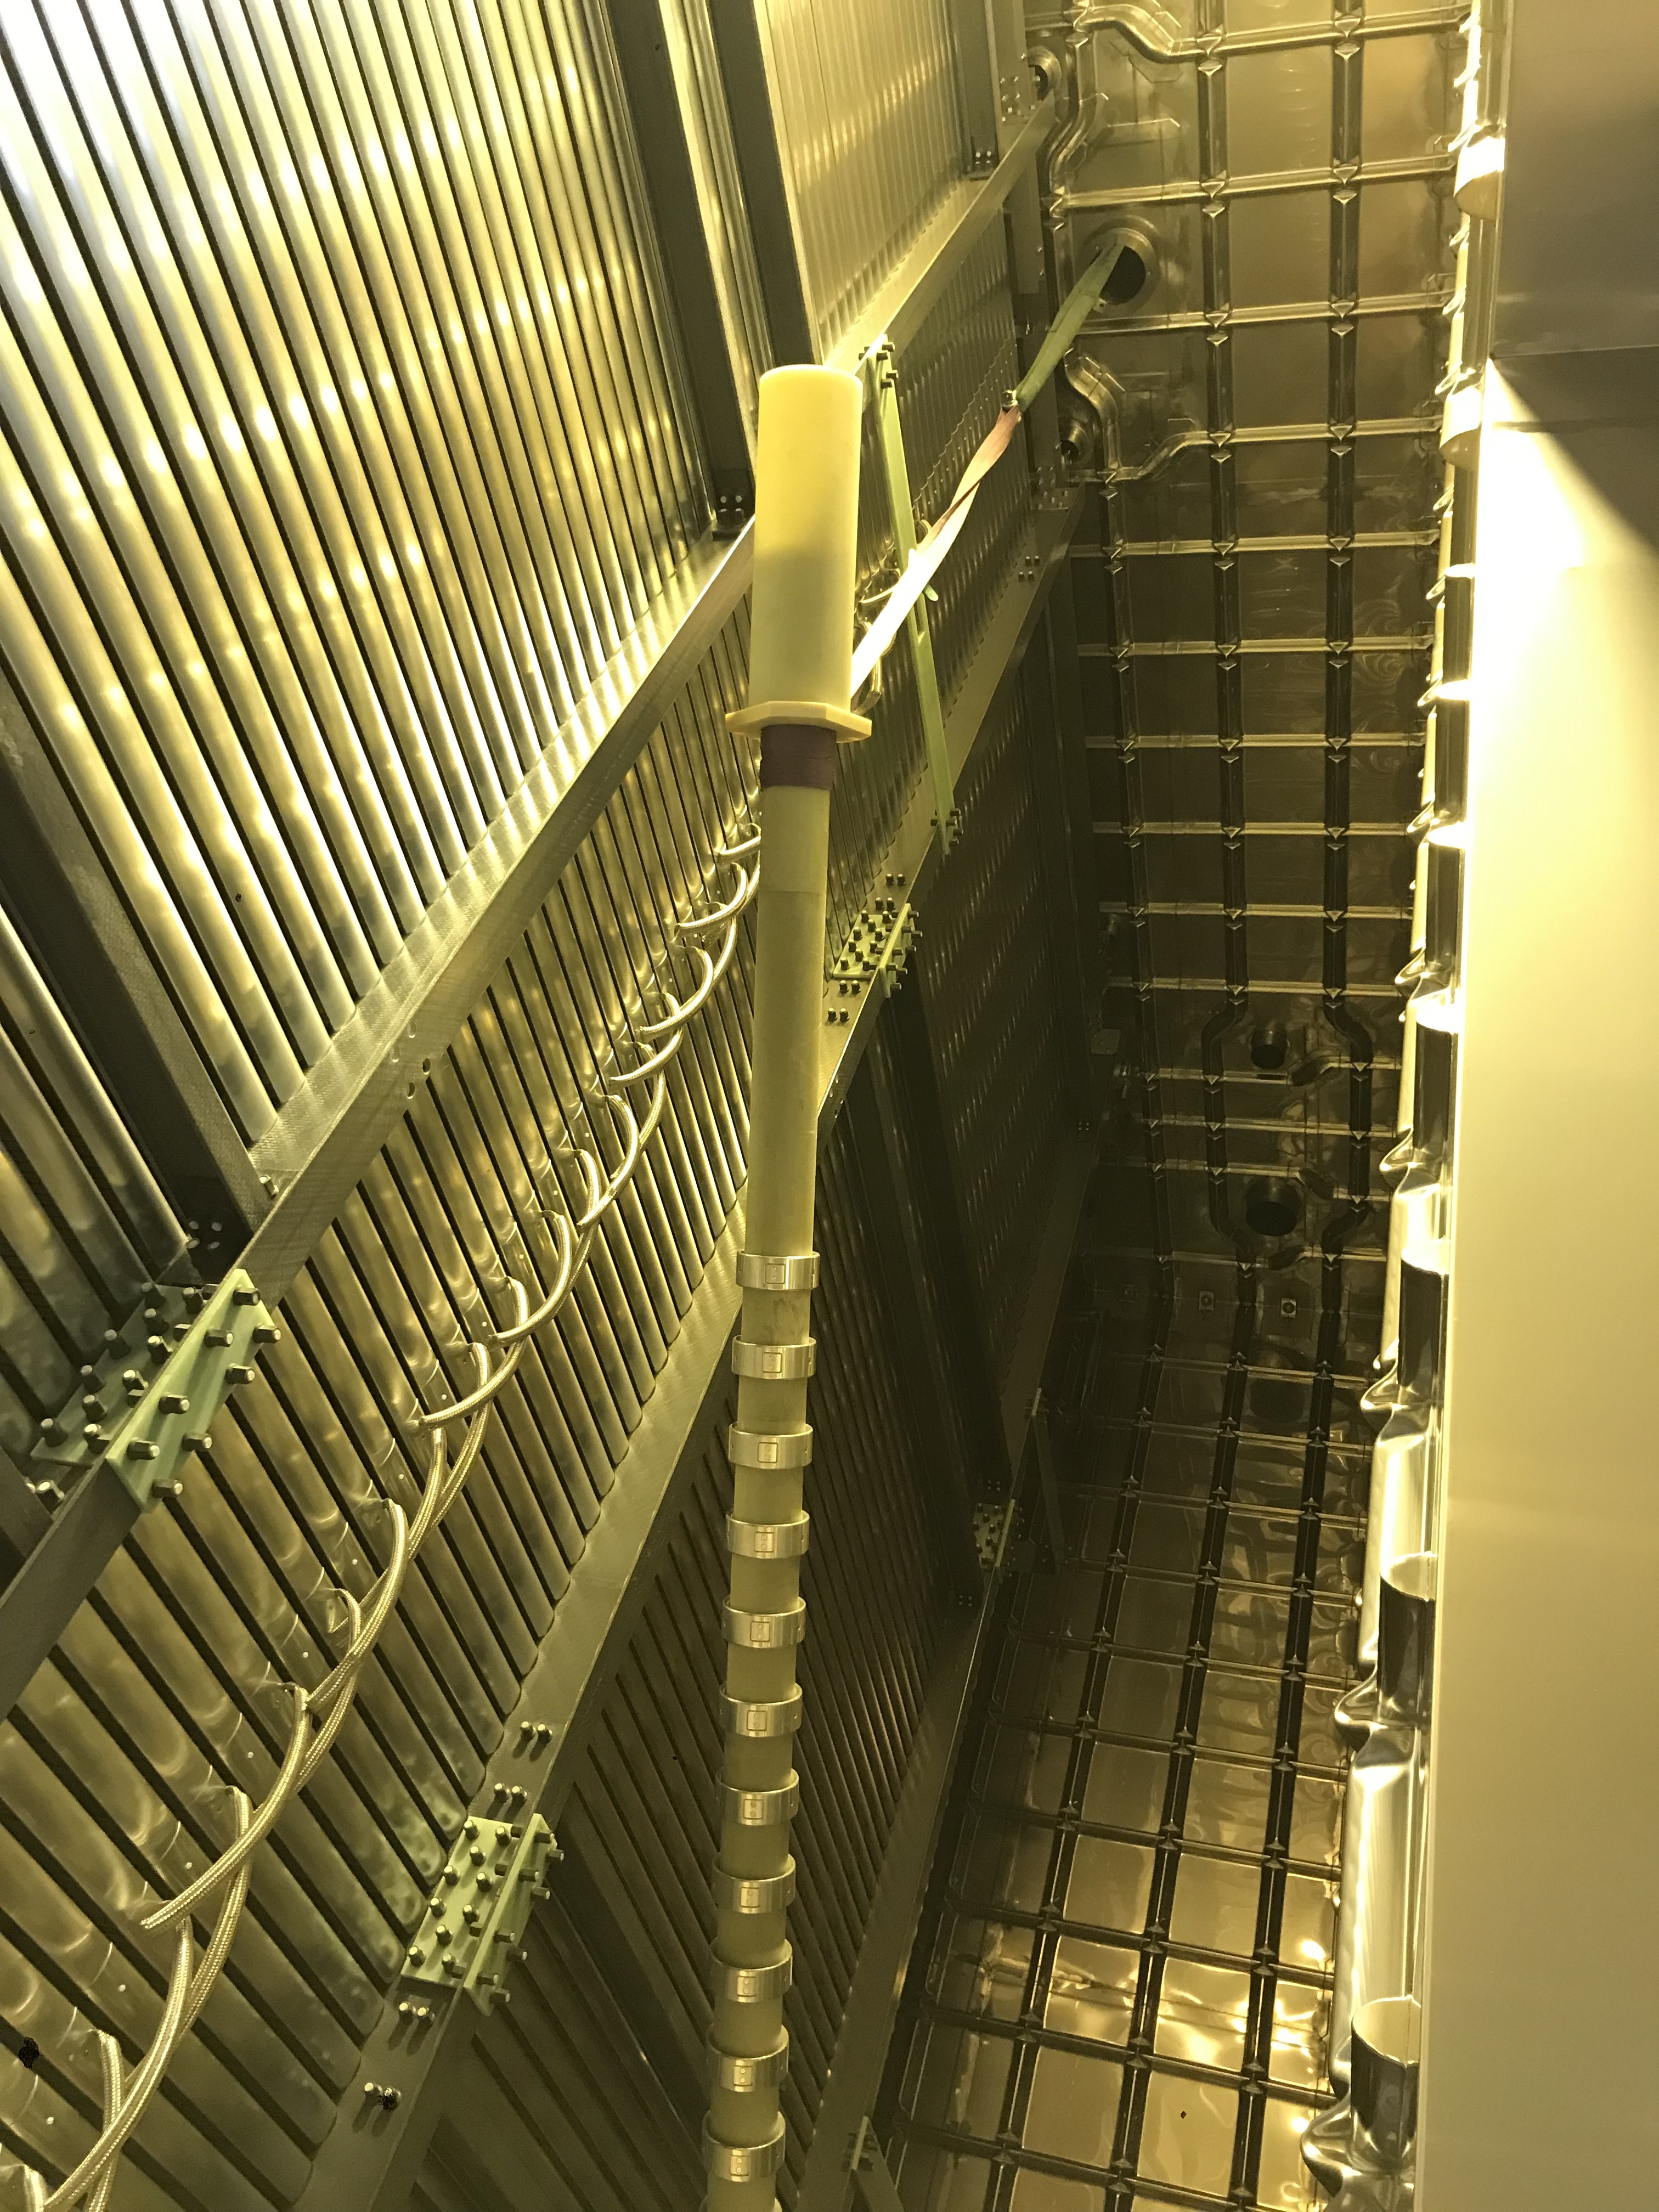
\includegraphics[width=0.9\textwidth]{extenderInstallation.jpg}
\end{dunefigure}



\subsection{Electronics installation}
The \dword{sgft} are installed and leak tested during the setup of the cryostat roof.
They must be available before the installation of the \dwords{crp} to connect the signal cables.
The \dword{fe} cards are mounted on the blades and inserted into the \dwords{sgft}.
The installation of the digital electronics and $\mu$TCA crates must be done once the infrastructure on the cryostat roof is completed.
This is mainly to prevent that ongoing work may damage the crates and the fibers connected to them.
Once the $\mu$TCA crates are installed and all the digital cards are inserted, the \dwords{amc} are cabled to the warm flanges of the \dword{sgft} for the charge readout, then connected to the \dword{pmt} signal cables for the light readout.
Finally, the 10~Gbit/s and 1~Gbit/s optical links to the \dword{daq} and \dword{wr} timing network are connected.

Given the presence of the cryogenic mezzanine and the unavailability of an overhead crane that can reach any position of the cryostat roof, the installation of the \dword{sgft} requires a compact gantry crane that can be moved on temporary rail or on wheels following the cryostat I-beams.
This part of installation will follow the welding of the corrugated membrane of the ceiling of the cryostat.
Sufficient amount of boxes containing the \dwords{sgft} must be stored underground.
The opening of the boxes is done on the cryostat roof.
After visual inspection, the \dwords{sgft} will be cleaned, hoisted with the gantry, inserted in the penetration and finally the CF flanges tightened.
Provided the availability of the material on the cryostat roof, two people can install eight \dwords{sgft} per shift. 
It will be crucial to test, possibly during the initial phase of the installation of the insulation that the penetrations are fulfill the requirements in terms of dimensions and linearity.
It is also important during the production of the \dword{sgft} to guarantee that all the pipes meet the requirements.
At \dword{pddp} the deformations of the penetration pipes due to welding and the dimensional non-conformity of few \dword{sgft} pipes resulted in delays of installation.
In parallel to the installation of the \dwords{sgft}, the \dword{fe} cards are unpacked on the cryostat roof, mounted on the blades on tables present for this purpose.
The instrumented blades are finally instrumented inserted in the \dword{sgft} before its sealing.
At this point, if the gas nitrogen pipes to purge the \dwords{sgft} are available they can be connected.
The sensors and the valves that potentially\footnote{It is not defined yet whether each \dword{sgft} needs independently temperature and pressures sensors and valves to control the gas nitroge flow.} needed to control the operation of the \dwords{sgft} can also be connected at this stage.
The installation of the $\mu$TCA crates with the digital electronics occurs in the final stage of the \dword{dpmod} installation to avoid damaging fragile equipment due to high level of co-activity expected on the cryostat roof for few months after the access to the top is granted.
The crates are placed and fixed in their designated positions on the cryostat roof.
They are connected to the power distribution network.
The \dword{amc} cards and \dword{wrmch} modules are inserted into their slots.
The connection of the \dword{cro} \dwords{amc} to the warm flange interface of the \dword{sgft} chimneys is done.
The optical fibres from the timing system are finally connected to the \dword{wrmch}.

The \dword{sgft} chimneys are commissioned first. This consists of evacuating their inner volume then filling the chimney with nitrogen gas at over-pressure between 5~mbar to 50~mbar.
The leak rate must be checked when the \dword{sgft} is under vacuum, and the nitrogen pressure must be monitored once the chimney is filled to verify that no damage occurs to the flange interfaces during installation.
Once the \dwords{sgft} are filled with gas nitrogen, the pressure must be constantly monitored and controlled.
It is crucial to monitor the \dword{sgft} pressure during the cryostat cool-down and filling.

The electronics system is commissioned after the $\mu$TCA crates,together with the \dwords{amc} and cabling the \dword{wr} network for the timing synchronization, are installed.
Functionality of the full \dword{daq} system is not strictly required at this stage.
The data from each crate is read with a portable computer connected to the crate using either the \dword{mch} 10~Gbit/s or 1~Gbit/s interface.
Non-functioning channels are identified by pulsing the CRP strips, and the data quality is examined to ensure the correct functioning of the digital electronics and the temporal alignment of the data segments.

\subsection{Light readout installation}

720~cryogenic Hamamatsu R5912-MOD20 \dwords{pmt}, below the transparent cathode structure, will be fixed on the membrane floor in the areas between the membrane corrugations.
The arrangement of the \dwords{pmt} accommodates the cryogenic piping on the membrane floor, and other elements installed in this area.
The attachment is done via a stainless steel support base point-glued to the membrane via four adhesive injection holes.
This fixation method will be long-term tested in cryogenic conditions prior the actual installation.
The installation of the \dword{pmt} will be done in sectors of 36~\dwords{pmt}, corresponding to the area below four \dwords{crp}, at a rate of 30~\dword{pmt}/week.
The \dwords{pmt} in each sectors will be installed, connected with cables and fibres, the connectivity will be tested, and finally the \dword{pmt} will be protected until the closure of the \dword{tco}. 

The \dwords{pmt} will be packed in individual boxes with their powering bases, support structures and short \dword{hv} cables soldered to the bases.
For shipping to \dword{ctsf} (probably located in the \dword{sdwf}), 36~\dwords{pmt} will then be placed in the transport boxes.
Following the \dword{ctsf} operations, the \dwords{pmt} will be placed in a custom structures in $4 \times 3$~arrays that can be moved into the clean room underground.
For transportation is done in boxes with three of these custom structures, for a total of 36~\dword{pmt} every box.
Excluding spares 20~boxes are needed to transport the 720~\dwords{pmt}.
The 80~spare \dwords{pmt} will be placed in three boxes, which can be stored in the \dword{ctsf}.
To maintain the cleanlyness inside the clean room underground, during tranportation the boxes will be wrapped with plastic that is then removed before entering into the clean room.
The entire $4 \times 3$ structure will go in the dark box for the final functionality tests.
The $4 \times 3$ array will be moved with the crane into the cryostat, placed on the cryostat floor, moved with trans-pallet at a convenient location for the installation, finally each \dwords{pmt} will be installed individually.

At the \dword{ctsf}, the \dwords{pmt} will be coated with \dword{tpb} at a rate of about 20~\dwords{pmt}/week.
The operations in the \dword{ctsf} should start enough in advance to secure sufficient availability of \dwords{pmt} during installation.
The \dword{ctsf} has sufficient storage capacity for the entire photon detector system of the \dword{dpmod}.

The weight of the support and the \dword{pmt} is approximately 7~kg.
Weight force exceeds the buoyancy force, still the assembly is light enough to be installed manually one at the time.
Given the large standing surface of the stainless steel plate, these supports ensure stability against possible lateral forces acting on the \dword{pmt}, for instance due to the liquid argon flow.

The support frame structure mainly comprises 304L stainless steel with some small Teflon parts.
The design takes into account the shrinking of the different materials during the cooling process to avoid breaking the \dword{pmt} glass.
The installation of an individual ground grids mechanically attached to the \dword{pmt} supports is also under consideration by the \dword{hv} and \dword{pd} system consortia.

Transport and storage of the cables and fibres are not an issue.
The cables and fibres arrive underground in boxes and they do not need to be cleaned before installation.
The cryostat cable/fiber installation will precede the installation of the \dword{fc}.
The cables/fibers will be routed from the relevant flanges to the bottom of the cryostat, with the help of dedicated cable trays and support from the cryogenic cooling pipes along the long walls.
Work at height will be carried out using the man lifts.
The free ends of the cables/fibers will be temporarily secured to the cryostat floor so they can be easily accessed during installation.
Once the temporary floor is removed, the ground grids set in high position and the \dwords{pmt} placed in their final position, the short \dword{hv} cables will be connected to the one coming from the feedthrough and the calibration fibers will be routed and connected to the support structure.
The fixation of the cables and fibres will be done at the level of the \dword{pmt} supports and on the ground grids.

\subsection{\dshort{tco} closure}
The activities related to the \dword{tco} closure involve heavy and dirty work, like grinding and welding, also inside the cryostat.
At that time, all the large detector components must be inside the cryostat including the material for the completion of the thermal insulation and the primary membrane.
The cryostat will be defined as a confined space, a work area with difficult egress.
The access will be limited and only from the available man-holes.
In order to access, scaffold is a solution being studied.
The height and the width of the volume between the \dword{fc} and the cryostat wall will require a special scaffold.
Alternatively, an electric pulley can be used to bring in and out material and personnel, by means of harness, that should anyway be used in a confined space.

Most of the detector will actually be installed, including the \dword{fc} end-wall in the proximity of the \dword{tco}.
This is the approach used in the \dword{pddp} case.
It is therefore mandatory to protect the cryostat, that should be considered as an ISO~8 class clean room, and the detector components.
A dirty room made out of aluminium profiles, plywood panels (treated with fire retardant agents) and fire retardant plastic sheets will be constructed in the area between the cryostat wall and the \dword{fc} end-wall.
Such a room was built in less than two week by four technicians inside the \dword{pddp}.
Since the access and the dirty room volume is similar to \dword{pddp}, the time and man power will be the same.
The engineering of the insulation and the primary membrane as not yet finalised, so the dimensions of the insulation panels and corrugated membrane needed for the \dword{tco} closure is not yet defined.
The dirty area anyway will be done large enough to store all the insulation panels needed.
They will be arranged in the correct installation order, because due to tight space it will be difficult to swap two panels.
The need of a scaffold in front of the \dword{tco} in order to be able to install the topmost panels is unavoidable.
The actual installation of the insulation and the primary membrane will most likely be carried out by the same company that installed the rest of the cryostat.
In the \dword{pddp} case this operation took less than four weeks and five people.
Again, the time estimation to complete this work in \dword{dpmod} is similar to the \dword{pddp} case.
The cleaning and the removal of the dirty room finally is done in the last two weeks dedicated to the \dword{tco} closure activities.

The last month of activities inside the cryostat is dedicated to complete the installation of the remaining cryogenic instrumentation, clean the cryostat and the accessible detector components, remove all the equipment needed for access and close finally the man-holes.


%\cleardoublepage

\section{Schedule}
\label{ch:dp-tc-schedrisk}

\fixme{Table~\ref{tab:Xsched} is a standard table template for the TDR schedules.  It contains overall FD dates from Eric James as of March 2019 (orange) that are held in macros in the common/defs.tex file so that the TDR team can change them if needed. Please do not edit these lines! Please add your milestone dates to fit in with the overall FD schedule. Please set captions and label appropriately. Anne}

\begin{dunefigure}[Overall installation schedule]{fig:overallSchedule}
{Overall installation schedule.}
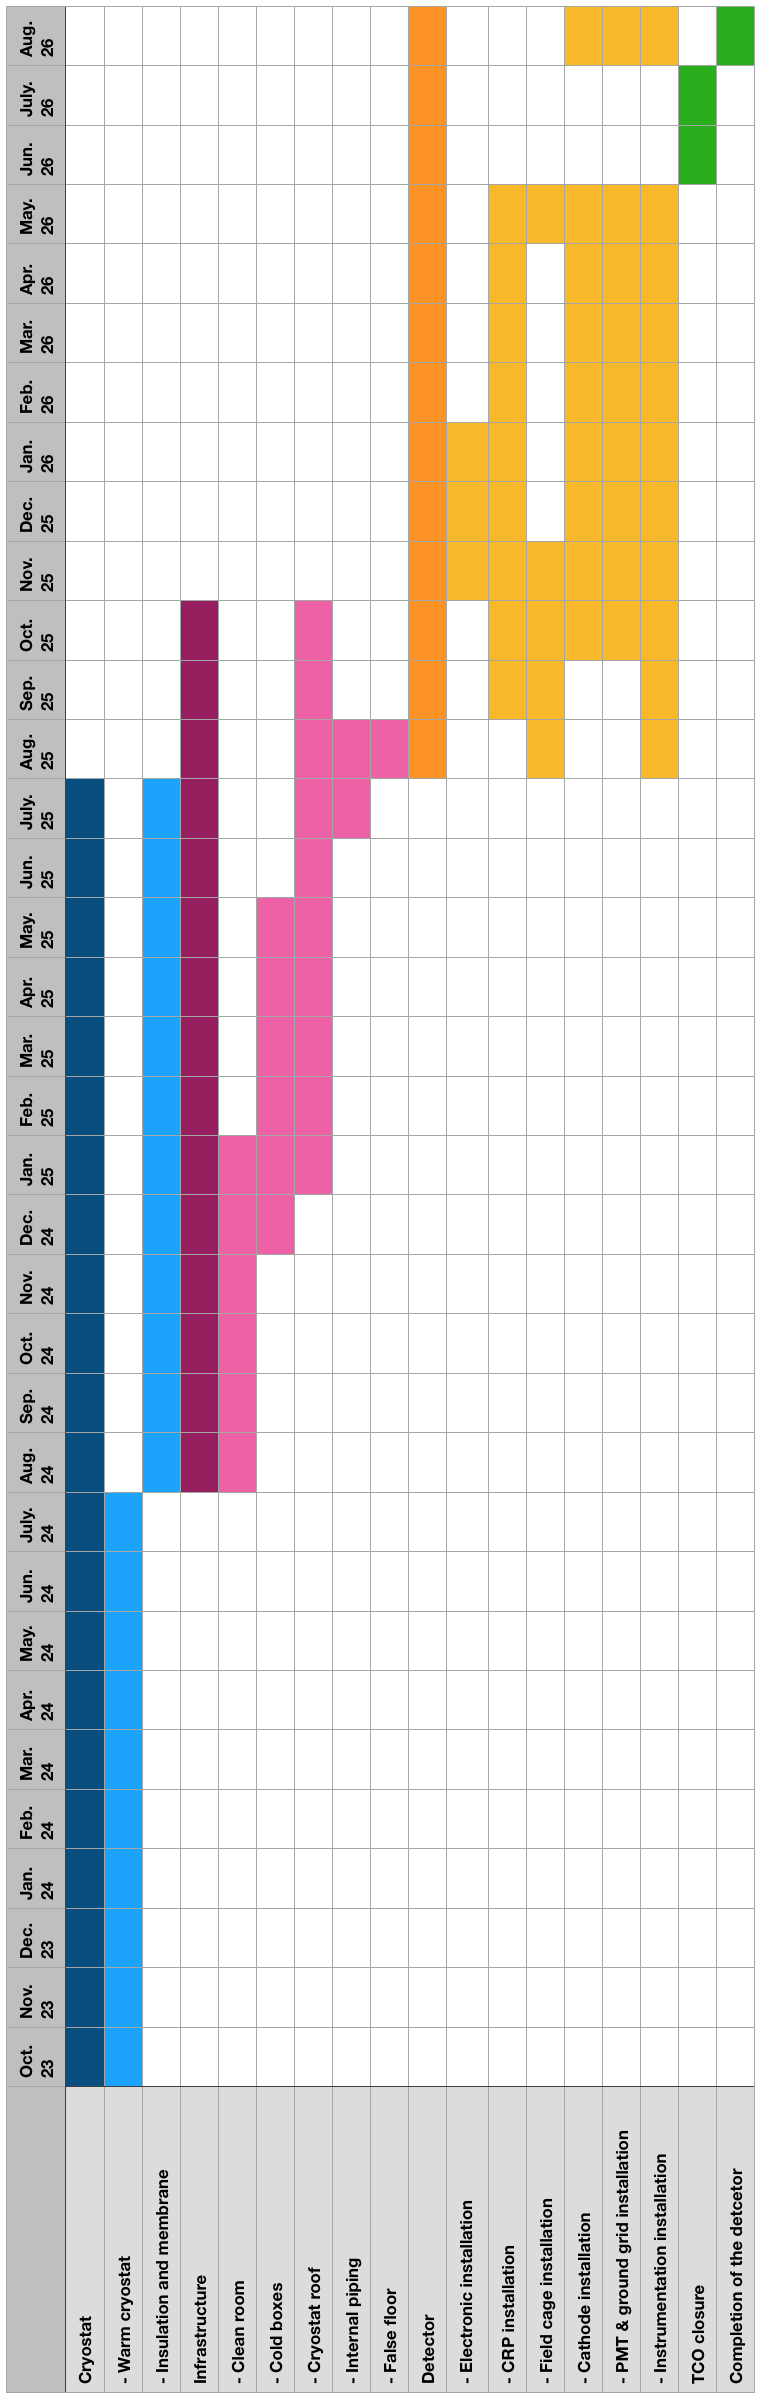
\includegraphics[width=0.4\textwidth]{overallSchedule.png}
\end{dunefigure}

Figure~\ref{fig:overallSchedule} show the overall schedule from the beginning of the warm cryostat construction to the closure of the man-holes.
In this schedule, the construction of the warm part of the \dword{dp} cryostat will take ten months, and will be done in parallel to the installation of the cold part of the \dword{sp} cryostat.
The insulation and the primary containment system of the \dword{dp} cryostat will follow.
Twelve months are dedicated to this activity done in parallel with the \dword{sp} detector installation and with the \dword{dp} infrastructure installation.
At most 144 people are allowed to be underground at anytime.
Six months are allocated for the construction of the clean room, structure, walls, overhead crane, ventilation, power and lighting systems. 
The installation priority in this period is given to the insulation and membrane: the construction of the clean room should not interfere or slow down the cold part of the cryostat.
Before the completion of the clean room, the construction of the cold boxes and the related cryogenic system must begin.
The time allocated for this activity is six months and it is believed that given the co-activity in the clean room at this time, the allocated time is just right.
In the mean time, the installation of the infrastructure on the cryostat roof must commence.
Ten months are dedicated to the welding of all the support structure, the penetration pipes and flanges, installation of the racks, cable trays, purge pipes, walk-able floor, \dword{crp} and \dword{fc} supports and the \dwords{sgft}.
These last three items must be ready before the beginning of the \dword{tpc} installation.
The electronics instalation can start when the first \dwords{sgft} are available.
Once the cryostat is complete, internal cryogenic piping and the false floor will be installed before the actual detector installation will begin.
As explained in the previous section, the cryogenic instrumentation and the \dword{fc} will be the items installed first.
The installation of all the \dword{fc} except for the last end-wall will be done in four months.
After cryogenic tests in the cold box the \dwords{crp} will be installed at a constant pace for nine months.
The cathode, ground grid and \dword{pmt} installation will follow the advances in the \dword{crp} installation.
The \dword{fc} end-wall and the \dword{hv} extender will be installed just after the last \dword{crp} is installed, connected and tested.
The \dword{tco} closure activities are scheduled for two months and the last months is dedicated to the final cleaning or the detector and the cryostat.
The table~\ref{tab:milestones} summarises the milestones for the \dword{dpmod} installation according to the global schedule just described.


\begin{dunetable}
[\dshort{dpmod} installation milestones]
{p{0.65\textwidth}p{0.25\textwidth}}
{tab:milestones}
{\dword{dpmod} installation milestones}   
Milestone & Date (Month YYYY)   \\ \toprowrule
Freeze roof penetration layout & March 2021 \\ \colhline
\rowcolor{dunepeach} Start of \dword{pdsp}-II installation& \startpduneiispinstall      \\ \colhline
Ash River installation tests complete & March 2022 \\ \colhline
\rowcolor{dunepeach} Start of \dword{pddp}-II installation& \startpduneiidpinstall      \\ \colhline
\rowcolor{dunepeach}South Dakota Logistics Warehouse available& \sdlwavailable      \\ \colhline
Installation Preliminary Design Review & September 2022 \\ \colhline
\rowcolor{dunepeach}Beneficial occupancy of cavern 1 and \dword{cuc}& \cucbenocc      \\ \colhline
\rowcolor{dunepeach} \dword{cuc} counting room accessible& \accesscuccountrm      \\ \colhline
Installation \dword{prr} & September 2023 \\ \colhline
Start production of infrastructure for Detector \#2 & October 2023 \\ \colhline
Start construction warm structure cryostat \#2 & October 2023 \\ \colhline
\rowcolor{dunepeach}Top of \dword{detmodule} \#1 cryostat accessible& \accesstopfirstcryo      \\ \colhline
\rowcolor{dunepeach}Start of \dword{detmodule} \#1 TPC installation& \startfirsttpcinstall      \\ \colhline
Start installation of cold structure Cryostat \#2 & August 2024 \\ \colhline
Start installation of infrastructure for Detector \#2 & August 2024 \\ \colhline
\rowcolor{dunepeach}Top of \dword{detmodule} \#2 accessible& \accesstopsecondcryo      \\ \colhline
\rowcolor{dunepeach}End of \dword{detmodule} \#1 TPC installation& \firsttpcinstallend      \\ \colhline
Start using the clean room & June 2025 \\ \colhline
\rowcolor{dunepeach}Start of \dword{detmodule} \#2 TPC installation& \startsecondtpcinstall      \\ \colhline
\rowcolor{dunepeach}End of \dword{detmodule} \#2 TPC installation& \secondtpcinstallend      \\ \colhline
\dword{tco} detector \#2 closed & August 2026 \\ \colhline
Start of cryogenic operation for detector \#2 & August 2026 \\ 
\end{dunetable}

